\documentclass[t]{beamer}

%-------------------------------------------------------------------------------
% 	colors
%-------------------------------------------------------------------------------
\usepackage{xcolor}
\definecolor{UBBlue}{cmyk}{1.0,0.7,0,0}
\definecolor{UBYellow}{cmyk}{0,0.3,1.0,0}
\definecolor{UBGray}{cmyk}{0,0,0.15,0.55}
\definecolor{UBBlueRGB}{RGB}{7,82,154}
\definecolor{UBYellowRGB}{RGB}{255,185,12}
\definecolor{UBGrayRGB}{RGB}{144,144,133}


%-------------------------------------------------------------------------------
% 	presentation setup
%-------------------------------------------------------------------------------
\mode<presentation>
{
    \usetheme{Boadilla}
    \useinnertheme{circles}
    \usecolortheme[named=UBBlue]{structure}

    % Adjust templates.
    \setbeamertemplate{navigation symbols}{} %Remove navigation symbols
	\setbeamertemplate{blocks}[rounded][shadow=false] % adjust blocks

    % Adjust colors.
    \setbeamercolor{author in head/foot}{bg=UBBlue, fg=white}
    \setbeamercolor{title in head/foot}{bg=UBYellow, fg=black}
    \setbeamercolor{date in head/foot}{bg=UBGray, fg=white}
    \setbeamercolor{title}{fg=UBBlue}
    \setbeamercolor{subtitle}{fg=UBGray}
	\setbeamercolor{institute}{fg=UBBlue}
    \setbeamercolor{author}{fg=UBBlue}
    \setbeamercolor{date}{fg=UBGray}
	\setbeamercolor{frametitle}{fg=UBBlue}
    \setbeamercolor{alerted text}{fg=UBBlue}
    \setbeamercolor{footnote mark}{fg=UBBlue}
    \setbeamercolor{footnote}{fg=UBBlue}
    \setbeamercolor{block title}{fg=black, bg=UBYellow}
    \setbeamercolor{block body}{fg=black, bg=UBGray!15}

    % Adjust page titles.
    \setbeamertemplate{frametitle}{%
        \vspace{3pt}%
        \parbox[c][1.0cm][b]{\textwidth}{%
            \usebeamerfont{frametitle}\usebeamercolor[fg]{frametitle}\insertframetitle%
						\hfill%
						\includegraphics[width=0.20\textwidth]{uni-bonn_mctc_logo.png}
        }
    }

    % Adjust footline.
    \setbeamertemplate{footline}
    {
      \hbox{%
      \begin{beamercolorbox}[wd=.333333\paperwidth,ht=2.5ex,dp=0.5ex,center]{author in head/foot}%
        \usebeamerfont{author in head/foot}\insertshortauthor
      \end{beamercolorbox}%
      \begin{beamercolorbox}[wd=.333333\paperwidth,ht=2.5ex,dp=0.5ex,center]{title in head/foot}%
        \usebeamerfont{title in head/foot}\insertshorttitle
      \end{beamercolorbox}%
      \begin{beamercolorbox}[wd=.283333\paperwidth,ht=2.5ex,dp=0.5ex,center]{date in head/foot}%
        \usebeamerfont{date in head/foot}\insertshortdate{}
      \end{beamercolorbox}%
      \begin{beamercolorbox}[wd=.05\paperwidth,ht=2.5ex,dp=0.5ex,right]{date in head/foot}%
        \usebeamerfont{date in head/foot}\insertframenumber{}\hspace*{2ex} 
      \end{beamercolorbox}}%
      \vskip0pt%
    }

    % Adjust fonts.
    \setbeamerfont{footnote}{size=\tiny}
	  \setbeamerfont{author in head/foot}{size=\tiny}
	  \setbeamerfont{title in head/foot}{size=\tiny}
	  \setbeamerfont{date in head/foot}{size=\tiny}
}


%-------------------------------------------------------------------------------
% 	layout, geometry
%-------------------------------------------------------------------------------
%\usepackage{enumitem}
%\setlist[itemize]{leftmargin=10pt}
\usepackage[absolute,overlay]{textpos}

\usepackage[%
	activate={true,nocompatibility}, % activate protrusion and expansion
	final, % enable microtype
	tracking=true,
	kerning=true,
	spacing=true,
	factor=1100, % add 10% to the protrusion amount (default is 1000)
	stretch=10, % 
	shrink=10, % reduce stretchability/shrinkability (default is 20/20)
	]{microtype}
\SetExtraKerning[unit=space]{%
	encoding={*},
	family={*},
	series={*},
	size={footnotesize,small,normalsize,scriptsize}}{
		"28={ ,150}, % left bracket, add space from right
		"29={150, }, % right bracket, add space from left
		\textquotedblleft={ ,150}, % left quotation mark, space from right
		\textquotedblright={150, } % right quotation mark, space from left
}
\SetTracking{encoding={*}, shape=sc}{40} % correct spacing for \textsc{}

\usepackage{layouts}          % for printing page width:
% textwidth in inches: \printinunitsof{in}\prntlen{\textwidth}


%-------------------------------------------------------------------------------
% 	language and time
%-------------------------------------------------------------------------------
\usepackage[T1]{fontenc}
\usepackage[utf8]{inputenc}\DeclareUnicodeCharacter{2212}{-}
\usepackage[american]{babel}
\microtypecontext{spacing=nonfrench} % extra space at end of sentence -> english
\usepackage[ddmmyyyy]{datetime}
\usepackage{bookmark}

%-------------------------------------------------------------------------------
% 	font
%-------------------------------------------------------------------------------
\newcommand\hmmax{0}
\newcommand\bmmax{0} 
\usepackage{lmodern}			% use lmodern font
\usepackage{upgreek}

%-------------------------------------------------------------------------------
% 	tables
%-------------------------------------------------------------------------------
\usepackage{tabularx}					% table with flexible column width
\usepackage{booktabs}                   % horizontal lines
\usepackage{float} 						% table placement
\usepackage{multirow} 					% multirow table

%-------------------------------------------------------------------------------
% 	figure, graphics
%-------------------------------------------------------------------------------
\usepackage[%
  singlelinecheck=true,
  justification=justified,
  format=plain,
  font=small,
  labelfont=it
]{caption}
\usepackage{subcaption}
\usepackage{graphicx}
\setbeamertemplate{caption}[numbered]
\graphicspath{{figures/}}

%-------------------------------------------------------------------------------
% 	math
%-------------------------------------------------------------------------------
\usepackage{amsmath,amsfonts,amsthm,amssymb,amstext}
\usepackage{bm}                           % for bold characters from greek alphabet
\usepackage{siunitx}
\sisetup{%
  detect-all,                             % alle äußeren Schriftkonventionen übernehmen
  per-mode=fraction,                      % \per creates fraction
  output-decimal-marker={.},              % decimal symbol 
  unit-mode=text,                         % Einheiten im Textmodus
  separate-uncertainty=true,              % von/bis oder \pm haben beide Einheit nach Zahl
  range-phrase=\ {\text{\textendash}}\ ,  % range denoted with endash (note spacing)
  range-units=single,                     % range has only one unit
  exponent-product=\cdot,                 % use \cdot: \SI{6,626E-34}{\joule\second}
  output-product=\cdot                    % use \cdot: \SI{6,626E-34}{\joule\second}
}       
\DeclareSIUnit{\calorie}{cal}
\DeclareSIUnit{\ppm}{ppm}
\DeclareSIUnit{\kcal}{\kilo\calorie}


%-------------------------------------------------------------------------------
% 	bibliography, citation, links
%-------------------------------------------------------------------------------
\usepackage[style=english]{csquotes} % required by biblatex.sty
\usepackage[backend=biber,style=chem-angew,maxbibnames=10,sorting=none]{biblatex} 
\addbibresource{literature.bib}



%-------------------------------------------------------------------------------
%   miscellaneous
%-------------------------------------------------------------------------------
\newcommand{\boltz}{k_{\mathsf{B}}}             % Boltzmann constant
\usepackage{lipsum}
\bmdefine{\balpha}{\alpha}                      % alpha in bold
\bmdefine{\bmu}{\upmu}                          % mu in bold and up (not italic)



%###############################################################################
%###############################################################################
%######################### !!!!! END OF PREAMBLE !!!!! #########################
%###############################################################################
%###############################################################################


%Einstellungen der Präsentation
\title[Vibrational Analysis and Spectroscopy]{Vibrational Analysis and Spectroscopy}
\subtitle{WP 8 Molecular Dynamics of Time-dependent Phenomena}
\author[T. Frömbgen, J. Blasius]{Tom Frömbgen and Jan Blasius}
\institute[MCTC]{Mulliken Center for Theoretical Chemistry, University of Bonn}
\date{25/10/2022}
\titlegraphic{
	\begin{center}
		\includegraphics[width=0.4\textwidth]{uni-bonn_mctc_logo.png}
	\end{center}
	
	\hspace{1.5cm}
	}

%Hier beginnt die Präsentation
\begin{document}
%%%%% Titelseite %%%%%%%%%%%%%%%%%%%%%%%%%%%%%%%%%%%%%%%%%%%%%%%%
\begin{frame}[noframenumbering,plain]
	\titlepage
\end{frame}
%%%%%%%%%%%%%%%%%%%%%%%%%%%%%%%%%%%%%%%%%%%%%%%%%%%%%%%%%%%%%%%%%
\begin{frame}
	\frametitle{Motivation}
	\begin{itemize}
		\item Molecules oscillate around equilibrium geometry
		\item Vibrations can be excited upon irradiation at proper wavelength
		\item Vibrational spectroscopy (IR, Raman) can be used for characterization and structure elucidation of compounds
		\item At ambient $T$, vibrations significantly contribute to thermodynamic properties
		\item[]
		      \pause
		\item Experimental measurements are (often) cost and time intensive
		\item Computation of vibrational modes of small molecules is fast and accurately possible today
	\end{itemize}
	\pause
	\begin{center}
		\textbf{How?}
	\end{center}
\end{frame}
%%%%%%%%%%%%%%%%%%%%%%%%%%%%%%%%%%%%%%%%%%%%%%%%%%%%%%%%%%%%%%%%%+
\begin{frame}{Potential energy surface (PES)}
	\begin{minipage}[b]{0.35\textwidth}
		\begin{itemize}
			\item We need to evaluate certain properties as functions of the nuclear coordinates
			\item Accurate modelling of the PES required
			\item Easiest model: 1D evaluation
		\end{itemize}
		\vspace{2.2cm}
	\end{minipage}
	\begin{minipage}[t]{0.6\textwidth}
		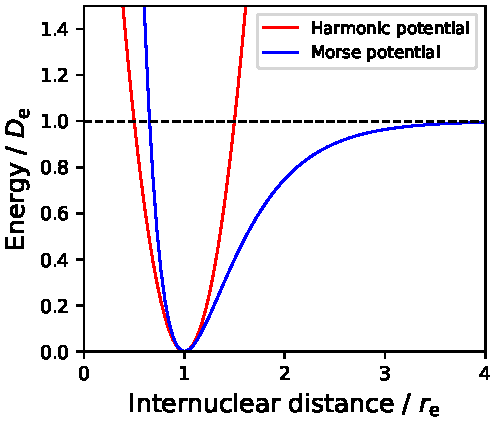
\includegraphics[width=\textwidth]{figures/potential.pdf}
	\end{minipage}
\end{frame}
%%%%%%%%%%%%%%%%%%%%%%%%%%%%%%%%%%%%%%%%%%%%%%%%%%%%%%%%%%%%%%%%%
\begin{frame}{PES modelling}
	\begin{enumerate}
		\item Static approach (QM)
		      \begin{itemize}
			      \item Solve stationary Schrödinger equation
			      \item[$+$] High accuracy (WFT, DFT)
			      \item[$+$] Fast
			      \item[$-$] Small region around (global) minimum geometry is modelled
		      \end{itemize}
		\item[]
		      \pause
		\item Dynamic approach (MD)
		      \begin{itemize}
			      \item Model time-dependent evolution of a system
			      \item Nuclear coordinates change, energy is evaluated along the trajectory
			      \item[$+$] Better sampling of the PES
			      \item[$+$] Good for liquid systems and solvation
			      \item[$-$] Often less accurate
			      \item[$-$] Computationally demanding
		      \end{itemize}
	\end{enumerate}
\end{frame}
%%%%%%%%%%%%%%%%%%%%%%%%%%%%%%%%%%%%%%%%%%%%%%%%%%%%%%%%%%%%%%%%%
\begin{frame}{Born--Oppenheimer approximation}
	We start from the Hamiltonian $\Hat{H}$ \pause
	\begin{equation*}
		\Hat{H} = \Hat{T}_\mathsf{e} + \Hat{T}_\mathsf{N} + \Hat{V}_\mathsf{eN} + \Hat{V}_\mathsf{ee} + \Hat{V}_\mathsf{NN}
	\end{equation*}
	\pause
	\vspace{-1cm}
	\begin{align*}
		\Hat{H} = & - \sum_i^n \frac{1}{2} \vec{\nabla}_i^2 - \sum_I^N \frac{1}{2M_i} - \sum_i^n \sum_I^N \frac{Z_I}{\left| \mathbf{r}_i-\mathbf{R}_I \right|}                              \\
		          & + \sum_i^{n-1} \sum_{j=i+1}^n \frac{1}{\left| \mathbf{r}_i-\mathbf{r}_j \right|} + \sum_I^{N-1} \sum_{J=I+1}^N \frac{Z_I Z_J}{\left| \mathbf{R}_i-\mathbf{R}_J \right|}
	\end{align*}
	and assume electrons to instantaneously adjust to the nuclear movement. Hence, we assume $\hat{T}_\mathsf{N}=0$ and $\hat{V}_\mathsf{NN}=\mathsf{const.}$, ending up at the electronic Hamiltonian $\hat{H}_\mathsf{el}$ \pause
	\begin{equation*}
		\hat{H}_\mathsf{el} = \Hat{T}_\mathsf{e} + \Hat{V}_\mathsf{eN} + \Hat{V}_\mathsf{ee}~.
	\end{equation*}
\end{frame}
%%%%%%%%%%%%%%%%%%%%%%%%%%%%%%%%%%%%%%%%%%%%%%%%%%%%%%%%%%%%%%%%%
\begin{frame}{Schrödinger equation}
	Using the electronic Hamiltonian, the electronic Schrödinger equation
	\begin{equation*}
		\hat{H}_\mathsf{el}(\mathbf{r,R}) \Psi_\mathsf{el}(\mathbf{r,R}) = E_\mathsf{el}(\mathbf{R}) \Psi_\mathsf{el}(\mathbf{r,R})
	\end{equation*}
	can be formulated. It depends \textit{explicitly} on the electronic coordinates but \textit{parametrically} on the nuclear coordinates.
	\newline
	\newline
	This problem is well known and can be solved for a given nuclear configuration (solving a stationary problem). Sampling of the PES in increments of $\Delta \mathbf{R}$ requires a lot of QM calculations.
	\newline
	\newline
	$\Longrightarrow$ too expensive!
\end{frame}
%%%%%%%%%%%%%%%%%%%%%%%%%%%%%%%%%%%%%%%%%%%%%%%%%%%%%%%%%%%%%%%%%
\begin{frame}{Nuclear Schrödinger equation I}
	We reinsert the kinetic energy of the nuclei and obtain the nuclear Schrödinger equation:
	\begin{equation*}
		(\hat{T}_\mathsf{N} + E_\mathsf{el}) \Psi = E\Psi~.
	\end{equation*}
	When recalling that the nuclei oscillate around the equilibrium geometry $R_0$, $E_\mathsf{el}$ is calculated only once. In the close vicinity it is approximated by a Taylor expansion of $E_\mathsf{el}$, which is truncated after the second term:
	\begin{equation*}
		V(\mathbf{R}) = E_\mathsf{el}(\mathbf{R_0}) + \left( \frac{\mathsf{d} E_\mathsf{el}}{\mathsf{d} \mathbf{R}}\right)^T (\mathbf{R - R_0}) + \frac{1}{2}(\mathbf{R - R_0})^T \left( \frac{\mathsf{d} E_\mathsf{el}^2}{\mathsf{d}^2 \mathbf{R}}\right) (\mathbf{R - R_0})~.
	\end{equation*}
	The terms $\left( \frac{\mathsf{d} E_\mathsf{el}^n}{\mathsf{d}^n \mathbf{R}}\right)$ are $3N \times 3N$ matrices. $E_\mathsf{el}(\mathbf{R_0})$ is chosen as reference energy and therefore, vanishes. $\mathbf{R_0}$ is a stationary point, hence $\left( \frac{\mathsf{d} E_\mathsf{el}}{\mathsf{d} \mathbf{R}}\right) = 0$. We define $\Delta \mathbf{R = R - R_0}$ and the second derivatives as force constant matrix $\mathbf{F}$.
\end{frame}
%%%%%%%%%%%%%%%%%%%%%%%%%%%%%%%%%%%%%%%%%%%%%%%%%%%%%%%%%%%%%%%%%
\begin{frame}{Nuclear Schrödinger equation II}
	The above expression simplifies to
	\begin{equation*}
		\left( -\sum_i^{3N} \frac{1}{2M_i}\frac{\partial^2}{\partial \mathsf{R}_i^2} + \frac{1}{2}\Delta \mathbf{R}^T \mathbf{F} \Delta \mathbf{R} \right) \Psi = E \Psi~,
	\end{equation*}
	which is well known as the harmonic oscillator. For the one-dimensional case, this expression can be written as \pause
	\begin{equation*}
		\left( -\frac{1}{2\mu}\frac{\mathsf{d}}{\mathsf{d}x} + \frac{1}{2}kx^2 \right) \Psi = E \Psi~.
	\end{equation*}
	Next, mass-weighted coordinates $\mathbf{y}$ are introduced as
	\begin{equation*}
		\mathsf{y}_i = \sqrt{M_i}\Delta \mathsf{R}_i~,~
		\frac{\partial^2}{\partial\mathsf{y}_i^2} = \frac{1}{M_i}\frac{\partial^2}{\partial\mathsf{R}_i^2}~.
	\end{equation*}
\end{frame}
%%%%%%%%%%%%%%%%%%%%%%%%%%%%%%%%%%%%%%%%%%%%%%%%%%%%%%%%%%%%%%%%%
\begin{frame}{Mass-weighted nuclear Schrödinger equation}
	Along with this, the force constant matrix $\mathbf{F}$ is also transformed into a mass-weighted form $\mathbf{F'}$
	\begin{equation*}
		\mathsf{F'_{ij}} = \frac{\mathsf{F}_{ij}}{\sqrt{M_i M_j}}~,
	\end{equation*}
	yielding a nuclear Schrödinger equation of the form
	\begin{equation*}
		\left( -\sum_i^{3N} \frac{1}{2}\frac{\partial^2}{\partial \mathsf{y}_i^2} + \frac{1}{2} \mathbf{y}^T \mathbf{F'}  \mathbf{y} \right) \Psi = E \Psi~.
	\end{equation*}
	This is a $3N$-dimensional problem because the dimensions are coupled via $\mathbf{F}$. To uncouple the differential equations, $\mathbf{F}$ must be diagonalized (removing all off-diagonal elements). The diagonalization is achieved by a unitary transformation which corresponds to a rotation of the coordinate system.
\end{frame}
%%%%%%%%%%%%%%%%%%%%%%%%%%%%%%%%%%%%%%%%%%%%%%%%%%%%%%%%%%%%%%%%%
\begin{frame}{Unitary transformation}
	With the unitary matrix $\mathbf{U}$, the coordinates are transformed:
	\begin{equation*}
		\mathbf{q = Uy}~,
	\end{equation*}
	which leads to a reformulated nuclear Schrödinger equation:
	\begin{equation*}
		\left( -\sum_i^{3N} \frac{1}{2}\frac{\partial^2}{\partial \mathsf{q}_i^2} + \frac{1}{2} \mathbf{q}^T \mathbf{UF'U}^T  \mathbf{q} \right) \Psi = E \Psi~.
	\end{equation*}
	The diagonalized force constant matrix $\mathbf{UF'U}$ is termed Hessian matrix $\mathbf{H}$, not to be confused with the Hamiltonian $\hat{H}$:
	\begin{equation*}
		\left( -\sum_i^{3N} \frac{1}{2}\frac{\partial^2}{\partial \mathsf{q}_i^2} + \frac{1}{2} \mathbf{q}^T \mathbf{H}  \mathbf{q} \right) \Psi = E \Psi~.
	\end{equation*}
\end{frame}
%%%%%%%%%%%%%%%%%%%%%%%%%%%%%%%%%%%%%%%%%%%%%%%%%%%%%%%%%%%%%%%%%
\begin{frame}{Separation into one-dimensional problems}
	As the Hessian $\mathbf{H}$ is diagonal in the transformed coordinate system, the vectors $\mathbf{q}$ are the eigenvectors of $\mathbf{H}$, \pause
	\begin{equation*}
		\mathbf{H}q_i = \lambda_i q_i~.
	\end{equation*}
	Inserting this into the nuclear Schrödinger equation, we end up at
	\begin{equation*}
		-\sum_i^{3N} \left( \frac{1}{2}\frac{\partial^2}{\partial \mathsf{q}_i^2} + \frac{1}{2} \lambda_i \mathbf{q}_i^2 \right) \Psi = E \Psi~.
	\end{equation*}
	This is analogue to $3N$ uncoupled one-dimensional harmonic oscillator problems:
	\begin{equation*}
		\left( -\frac{1}{2\mu}\frac{\mathsf{d}}{\mathsf{d}x} + \frac{1}{2}kx^2 \right) \Psi = E \Psi~.
	\end{equation*}
\end{frame}
%%%%%%%%%%%%%%%%%%%%%%%%%%%%%%%%%%%%%%%%%%%%%%%%%%%%%%%%%%%%%%%%%
\begin{frame}{Vibrational frequencies}
	As a last step, the vibrational frequencies $\nu_i$ can be derived analogously to the harmonic oscillator $\nu_i^{HO}$ \pause
	\begin{align*}
		\nu_i^{HO} = & \frac{1}{2\pi}\sqrt{\frac{k}{\mu}}~, \\
		\nu_i =      & \frac{1}{2\pi}\sqrt{\lambda_i}~.
	\end{align*}
	In practice, five or six eigenvalues of the Hessian are 0 \pause because these correspond to the translational and rotational degrees of freedom. Negative eigenvalues proof the stationary geometry to be a saddle point. If all eigenvalues are positive, a true minimum of the PES was found.
\end{frame}
%%%%%%%%%%%%%%%%%%%%%%%%%%%%%%%%%%%%%%%%%%%%%%%%%%%%%%%%%%%%%%%%%
\begin{frame}{Spectroscopic Intensities I}
	Most QC codes available today rely on the \textit{double harmonic approximation}:
	\begin{enumerate}
		\item All vibrational modes are assumed as harmonic oscillators
		\item The fundamental properties describing the spectroscopic intensities are determined by the first-order geometric derivative of the polarization property governing the spectroscopic phenomenon under study \\
	\end{enumerate}
	$\longrightarrow$ IR: \pause molecular electric dipole moment $\bmu$ \\
	$\longrightarrow$ Raman: \pause molecular polarizability $\balpha$
\end{frame}
%%%%%%%%%%%%%%%%%%%%%%%%%%%%%%%%%%%%%%%%%%%%%%%%%%%%%%%%%%%%%%%%%
\begin{frame}{IR Intensities I}
	From basic QC, we invoke that the transition rate $W_{k\rightarrow f}$ from an initial state $|k\rangle$ to a final state $|f\rangle$ induced by a perturbation operator $\hat{H}'$ reads \pause
	\begin{equation*}
		W_{k\rightarrow f}\propto \left| \langle f | \hat{H}' | k \rangle \right|^2~.
	\end{equation*}
	The system is perturbed by electromagnetic radiation (e.g. IR). The perturbation is approximated as a dipole, meaning
	\begin{equation*}
		\hat{H}' = - \langle \mathsf{e_g} | \bmu\mathbf{E} | \mathsf{e_g} \rangle
		= - \langle \mathsf{e_g} | \bmu | \mathsf{e_g} \rangle \mathbf{E_0}
		= - \bmu(\mathbf{q}) \mathbf{E_0}~,
	\end{equation*}
	while assuming the electric field $\mathbf{E}$ to be constant over the extent of the molecule. The dipole moment is obtained as a function of the nuclear coordinates $\bmu(\mathbf{q})$ by calculating the expectation value with the electronic ground state $| \mathsf{e_g} \rangle$.
\end{frame}
%%%%%%%%%%%%%%%%%%%%%%%%%%%%%%%%%%%%%%%%%%%%%%%%%%%%%%%%%%%%%%%%%
\begin{frame}{IR Intensities II}
	The dipole moment is then expanded in a Taylor series up to first order:
	\begin{equation*}
		\bmu(\mathbf{q}) = \bmu_0 + \sum_{i=1}^{3N-6} \left( \frac{\partial\bmu(\mathbf{q})}{\partial \mathsf{q}_i} \right) \mathsf{q}_i~.
	\end{equation*}
	When inserting analytical expressions for this term, we end up at the following expression for the absorption coefficients $A_i$ for the vibrational modes $i$ of the fundamental excitation:
	\begin{equation*}
		A_i = \frac{N_\mathsf{A}}{12\epsilon_0c^2} \left( \frac{\partial\bmu(\mathbf{q})}{\partial \mathsf{q}_i} \right)^2~.
	\end{equation*}
	This shows, that only those vibrational modes which cause a change of the molecular dipole moment along the mode, show up in the IR spectrum.
\end{frame}
%%%%%%%%%%%%%%%%%%%%%%%%%%%%%%%%%%%%%%%%%%%%%%%%%%%%%%%%%%%%%%%%%
\begin{frame}{Raman Intensities I}
	For the Raman intensities, a similar approach is used: According to the Placzek classical theory of polarization, the electric field induces a dipole moment $\bmu^\mathsf{ind}$ in the molecule and the Intensity $I$ is proportional to
	\begin{equation*}
		I \propto \left| \langle \bmu^\mathsf{ind} \rangle \right|^2~,
	\end{equation*}
	\begin{equation*}
		\langle \bmu^\mathsf{ind} \rangle = \langle f | \balpha(\mathbf{q}) | k \rangle \mathbf{E_0}~.
	\end{equation*}
	with the initial and final states $|k\rangle,|f\rangle$ and the assumption of a constant electric field $E$ over the extend of the molecule. The molecular polarizability $\balpha(\mathbf{q})$ is expanded in a Taylor series up to the first order:
	\begin{equation*}
		\balpha(\mathbf{q}) = \balpha_0 + \sum_{i=1}^{3N-6} \left( \frac{\partial\balpha(\mathbf{q})}{\partial \mathsf{q}_i} \right) \mathsf{q}_i~.
	\end{equation*}
\end{frame}
%%%%%%%%%%%%%%%%%%%%%%%%%%%%%%%%%%%%%%%%%%%%%%%%%%%%%%%%%%%%%%%%%
\begin{frame}{Raman Intensities II}
	After inserting analytical expressions for the respective terms, we yield the intensities $I_i$ for the vibrational modes $i$. In experimental Raman spectroscopy, the scattered intensities can be measured in different directions with respect to the incident beam:
	\begin{align*}
		I_i^\parallel = & C \frac{(\tilde{\nu}_\mathsf{in} - \tilde{\nu}_i)^4}{\tilde{\nu}_i (1- \exp\left(-\frac{hc\tilde{\nu}_i}{\boltz T}\right))} \left( \frac{\partial\balpha_{xx}(\mathbf{q})}{\partial \mathsf{q}_i} \right)^2~, \\
		I_i^\perp =     & C \frac{(\tilde{\nu}_\mathsf{in} - \tilde{\nu}_i)^4}{\tilde{\nu}_i (1- \exp\left(-\frac{hc\tilde{\nu}_i}{\boltz T}\right))} \left( \frac{\partial\balpha_{xy}(\mathbf{q})}{\partial \mathsf{q}_i} \right)^2~.
	\end{align*}
	This shows, that only those vibrational modes which cause a change of the molecular polarizability along the mode, show up in the Raman spectrum.
\end{frame}
%%%%%%%%%%%%%%%%%%%%%%%%%%%%%%%%%%%%%%%%%%%%%%%%%%%%%%%%%%%%%%%%%
%%%%%%%%%%%%%%%%%%%%%%%%%%%%%%%%%%%%%%%%%%%%%%%%%%%%%%%%%%%%%%%%%
\begin{frame}[plain,c]
	\frametitle{Molecular dynamics}
	\centering \Large
	Molecular Dynamics \\~\ vs. \\~\ Static Quantum Chemistry \\~\\
	What are the differences?
\end{frame}
%%%%%%%%%%%%%%%%%%%%%%%%%%%%%%%%%%%%%%%%%%%%%%%%%%%%%%%%%%%%%%%%%
\begin{frame}
	\frametitle{Spectroscopy in the liquid phase}
	\begin{figure}
		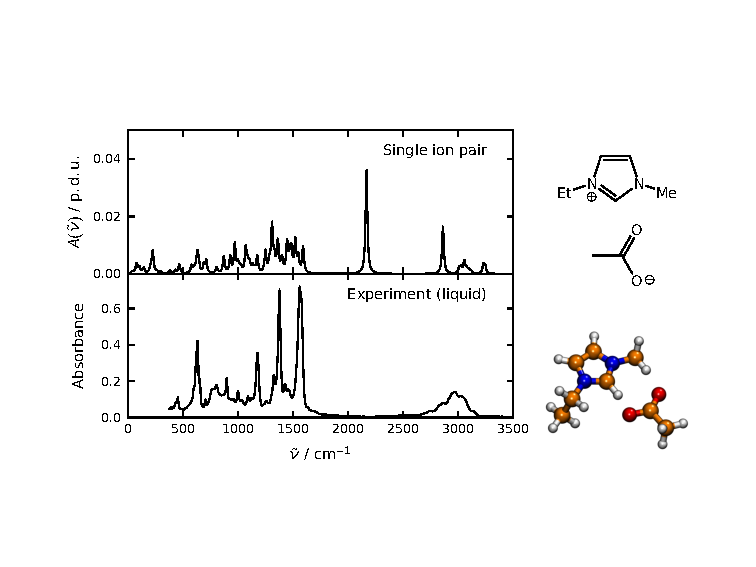
\includegraphics[width=0.85\textwidth]{figures/emimoac_ir.pdf}
	\end{figure}
	\pause
	\begin{itemize}
		\item Carbene formation in the gas phase
		\item isolated ion pair not sufficient to model the IR spectrum of the liquid phase
	\end{itemize}
\end{frame}
%%%%%%%%%%%%%%%%%%%%%%%%%%%%%%%%%%%%%%%%%%%%%%%%%%%%%%%%%%%%%%%%%
\begin{frame}
	\frametitle{Spectroscopy in the liquid phase}
	\begin{figure}
		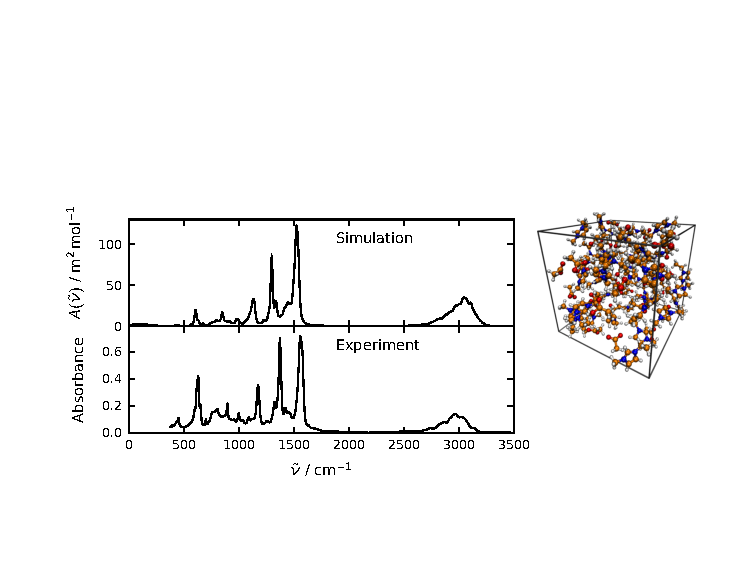
\includegraphics[width=\textwidth]{figures/emimoac_ir2.pdf}
	\end{figure}
	\begin{itemize}
		\item Calculate spectrum from AIMD simulation
		\item Accounts for explicit solvation effects, polarization, dynamics, anharmonicity and conformational averaging
	\end{itemize}
\end{frame}
%%%%%%%%%%%%%%%%%%%%%%%%%%%%%%%%%%%%%%%%%%%%%%%%%%%%%%%%%%%%%%%%%
\begin{frame}
	\frametitle{Green--Kubo approach}
	\begin{itemize}
		\item \textbf{Green--Kubo}:
		      \begin{itemize}\normalsize
			      \item MD provides time-dependent properties
			      \item Express time-dependent phenomena as integrals over correlation-functions
		      \end{itemize}
		\item[]
		      \pause
		\item \textbf{Correlation functions}:
		      \begin{itemize}\normalsize
			      \item Take data sets $x$ and $y$ and investigate which correlation exists between them
			            \begin{align*}
				            r_{xy} = \frac{\sum(x_i - \bar x)(y_i - \bar y)}{\sqrt{\sum(x_i - \bar x)^2 \sum (y_i - \bar y)^2}}
			            \end{align*}
			      \item Provides statistical relationship between variables
		      \end{itemize}
	\end{itemize}
\end{frame}
%%%%%%%%%%%%%%%%%%%%%%%%%%%%%%%%%%%%%%%%%%%%%%%%%%%%%%%%%%%%%%%%%
\begin{frame}
	\frametitle{Wiener--Khintchine theorem}
	\begin{itemize}
		\item Relates the Fourier transform of $f(t)$ to the autocorrelation function
		      \pause
		\item Autocorrelation function can be calculated by
		      \begin{itemize}\normalsize
			      \item 1. Taking the square of the absolute value of its Fourier transform
			            \begin{align*}\textcolor{lightgray}{
				            \langle C(\tau)C(t+\tau) \rangle_\tau = \frac{1}{2\pi} \int \textcolor{black}{\Bigg| \int f(t)\mathsf{e}^{-i\omega t}\mathsf{d}t \Bigg|^2} \mathsf{e}^{i\omega t}\mathsf{d}\omega}
			            \end{align*}
			            \pause
			      \item 2. Applying the inverse Fourier transform
			            \begin{align*}
				            \langle C(\tau)C(t+\tau) \rangle_\tau = \frac{1}{2\pi} \int \Bigg| \int f(t)\mathsf{e}^{-i\omega t}\mathsf{d}t \Bigg|^2 \mathsf{e}^{i\omega t}\mathsf{d}\omega
			            \end{align*}
		      \end{itemize}
		\item \textbf{Advantage}: Fast Fourier transform algorithms are faster than a direct computation of the autocorrelation function
	\end{itemize}
\end{frame}
%%%%%%%%%%%%%%%%%%%%%%%%%%%%%%%%%%%%%%%%%%%%%%%%%%%%%%%%%%%%%%%%%
\begin{frame}
	\frametitle{Correlation functions for vibrational spectra}
	\begin{itemize}
		\item \textbf{Infrared:}
		      \begin{align*}
			      A (\tilde{\nu}) \propto \int \langle \dot{\bmu} (\tau) \cdot \dot{\bmu} (t + \tau) \rangle_\tau \mathsf{e}^{-2\pi i c \tilde{\nu} t}\mathsf{d}t
		      \end{align*}
		      \pause
		\item \textbf{Raman:}
		      \begin{align*}
			      I (\tilde{\nu}) & \propto  \frac{(\tilde{\nu}_\mathsf{in}-\tilde{\nu})^4}{\tilde{\nu} \left( 1-\exp\left(-\frac{hc\tilde{\nu}}{\boltz T}\right)\right)} \\ & \times \int \left(\langle \dot{\balpha}_{xx}(\tau)\dot{\balpha}_{xx}(t + \tau) \rangle + \langle \dot{\balpha}_{xy}(\tau)\dot{\balpha}_{xy}(t + \tau) \rangle \right) \mathsf{e}^{-2\pi i c \tilde{\nu} t} \mathsf{d} t
		      \end{align*}
		      \pause
		\item \textbf{Vibrational circular dichroism:}
		      \begin{align*}
			      \Delta A (\tilde{\nu}) \propto \int \biggl[\langle \dot{\bmu} (\tau) \cdot \dot{\boldsymbol{\mathsf{m}}} (t + \tau) \rangle_{\tau} - \langle \dot{\boldsymbol{\mathsf{m}}} (\tau) \cdot \dot{\bmu} (t + \tau) \rangle_{\tau} \biggl] \mathsf{e}^{-2\pi i c \tilde{\nu} t}\mathsf{d}t
		      \end{align*}
	\end{itemize}
\end{frame}
%%%%%%%%%%%%%%%%%%%%%%%%%%%%%%%%%%%%%%%%%%%%%%%%%%%%%%%%%%%%%%%%%
\begin{frame}
	\frametitle{Wannier functions}
	\textbf{Dipole moment}
	\begin{itemize}
		\item Established approach: Maximally localized Wannier functions
		      \begin{figure}
			      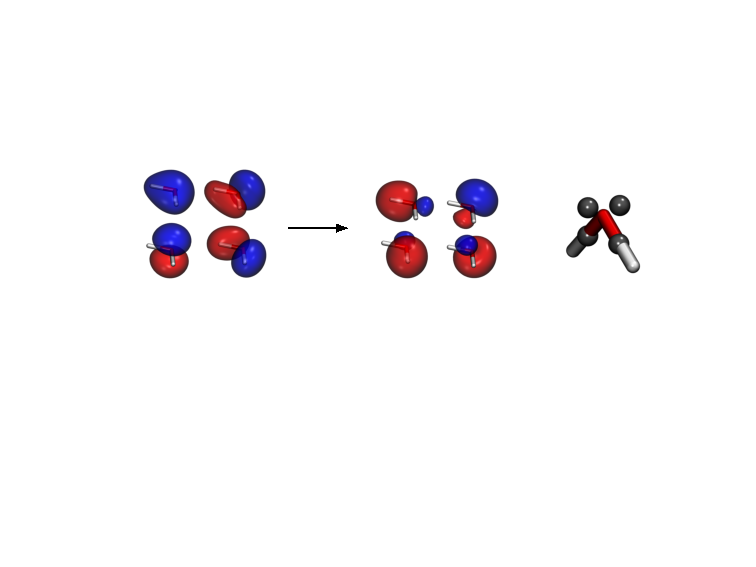
\includegraphics[width=0.6\textwidth]{figures/wannier.pdf}
		      \end{figure}
		\item Wannier function centers as locations of electron pairs
		\item Dipole moment as sum over point charges
		      \begin{align*}
			      \boldsymbol\upmu = -2e \sum_{i \in \mathsf{Wan.}} \mathbf{r}_i + e \sum_{j \in \mathsf{Nuc.}} Z_j \mathbf{R}_j
		      \end{align*}
	\end{itemize}
	\pause
	\textbf{Polarizability}
	\begin{itemize}
		\item Recalculate orbitals with external electric field
		      \begin{align*}
			      \boldsymbol\upmu_{\mathsf{ind}} = \balpha\mathbf{E}
		      \end{align*}
		\item Polarizability by finite differences
	\end{itemize}
\end{frame}
%%%%%%%%%%%%%%%%%%%%%%%%%%%%%%%%%%%%%%%%%%%%%%%%%%%%%%%%%%%%%%%%%
\begin{frame}
	\frametitle{Voronoi tessellation}
	\begin{figure}
		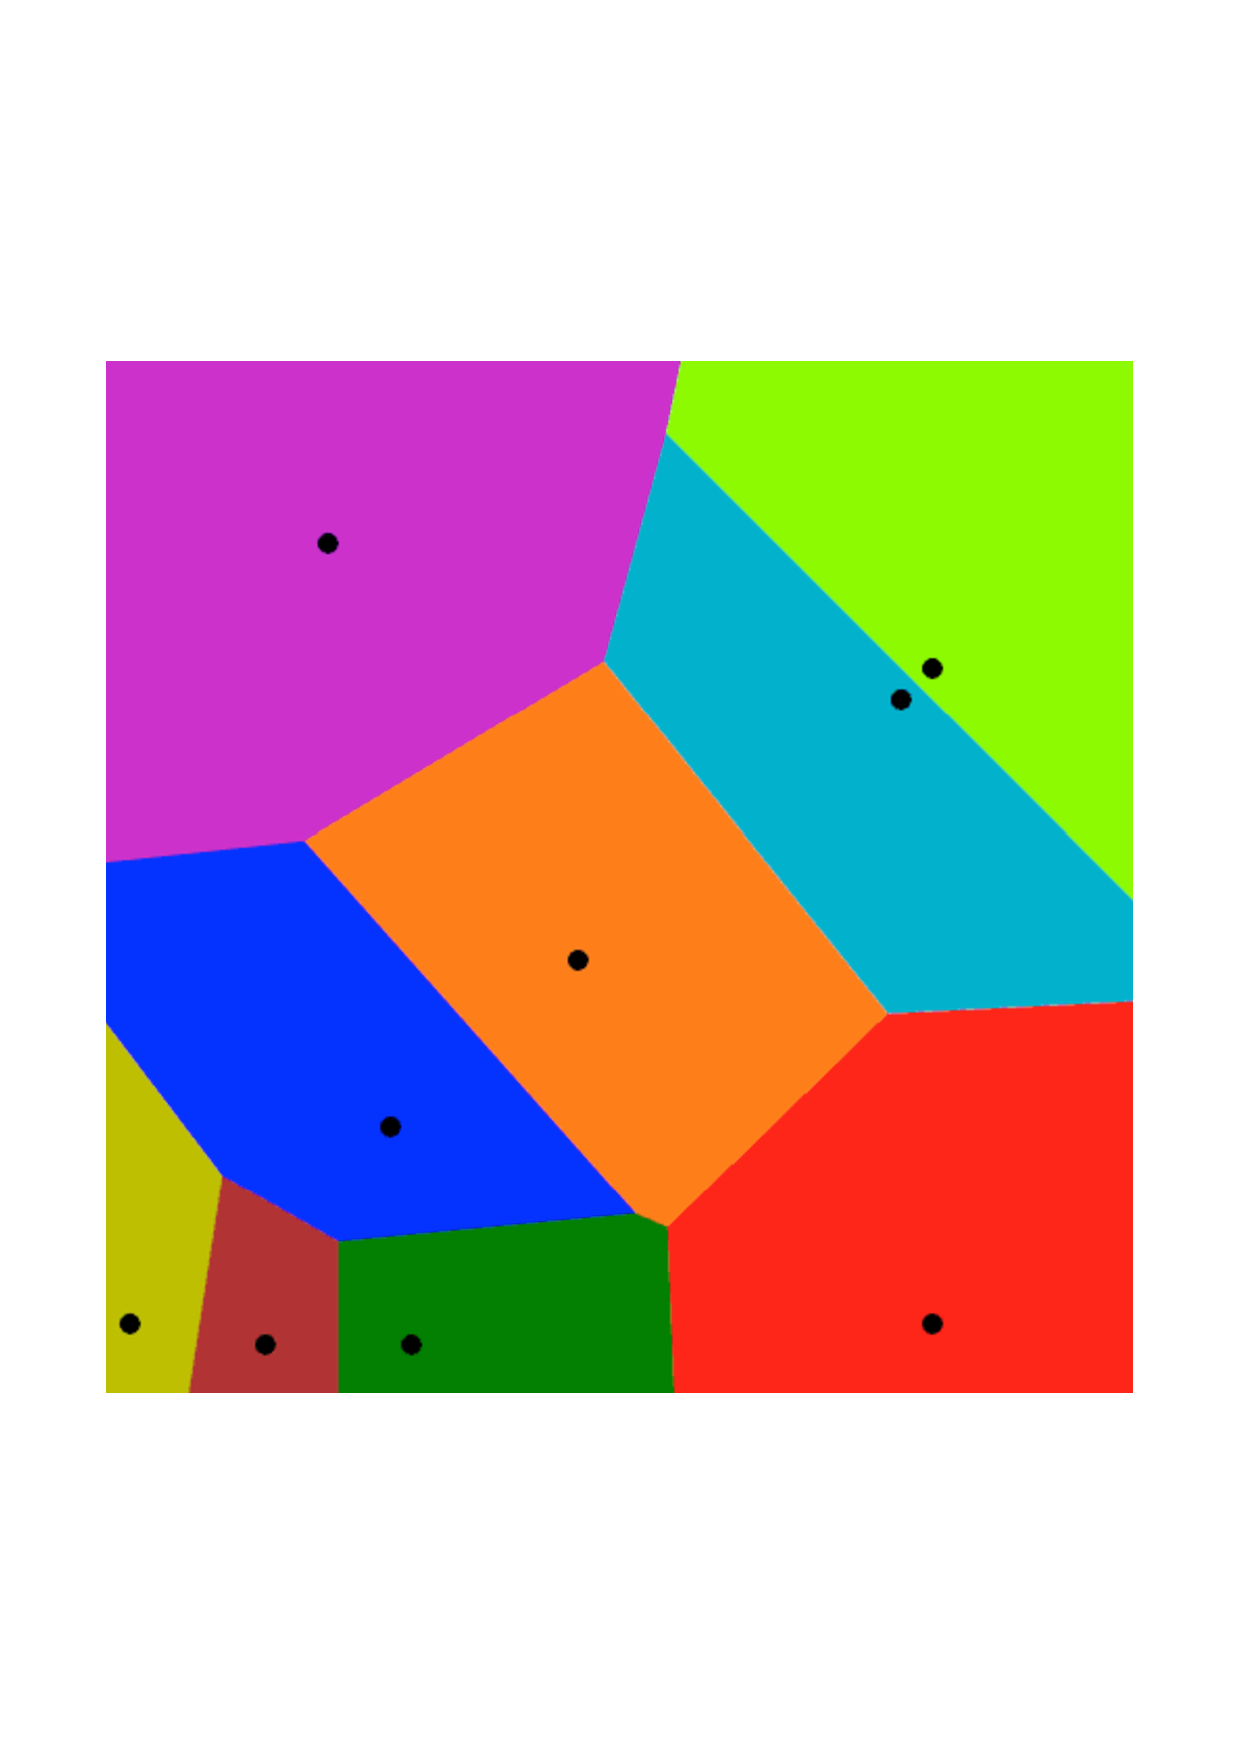
\includegraphics[width=0.4\textwidth]{figures/Voronoi.pdf}
	\end{figure}
	\begin{itemize}
		\item Division of Euclidean space into set of Voronoi cells
		\item Each point in space assigned to a site $s_i$ to which it is closest
		      \begin{align*}
			      C_i = \{ \mathbf{x} \in \mathbb{R}^3 \, | ( \mathbf{x} - \mathbf{s}_i )^2 \leq ( \mathbf{x} - \mathbf{s}_j )^2 \, \forall \, j \neq i \}; i,j=1,...,n
		      \end{align*}
	\end{itemize}
\end{frame}
%%%%%%%%%%%%%%%%%%%%%%%%%%%%%%%%%%%%%%%%%%%%%%%%%%%%%%%%%%%%%%%%%
\begin{frame}
	\frametitle{Voronoi tessellation}
	\begin{figure}
		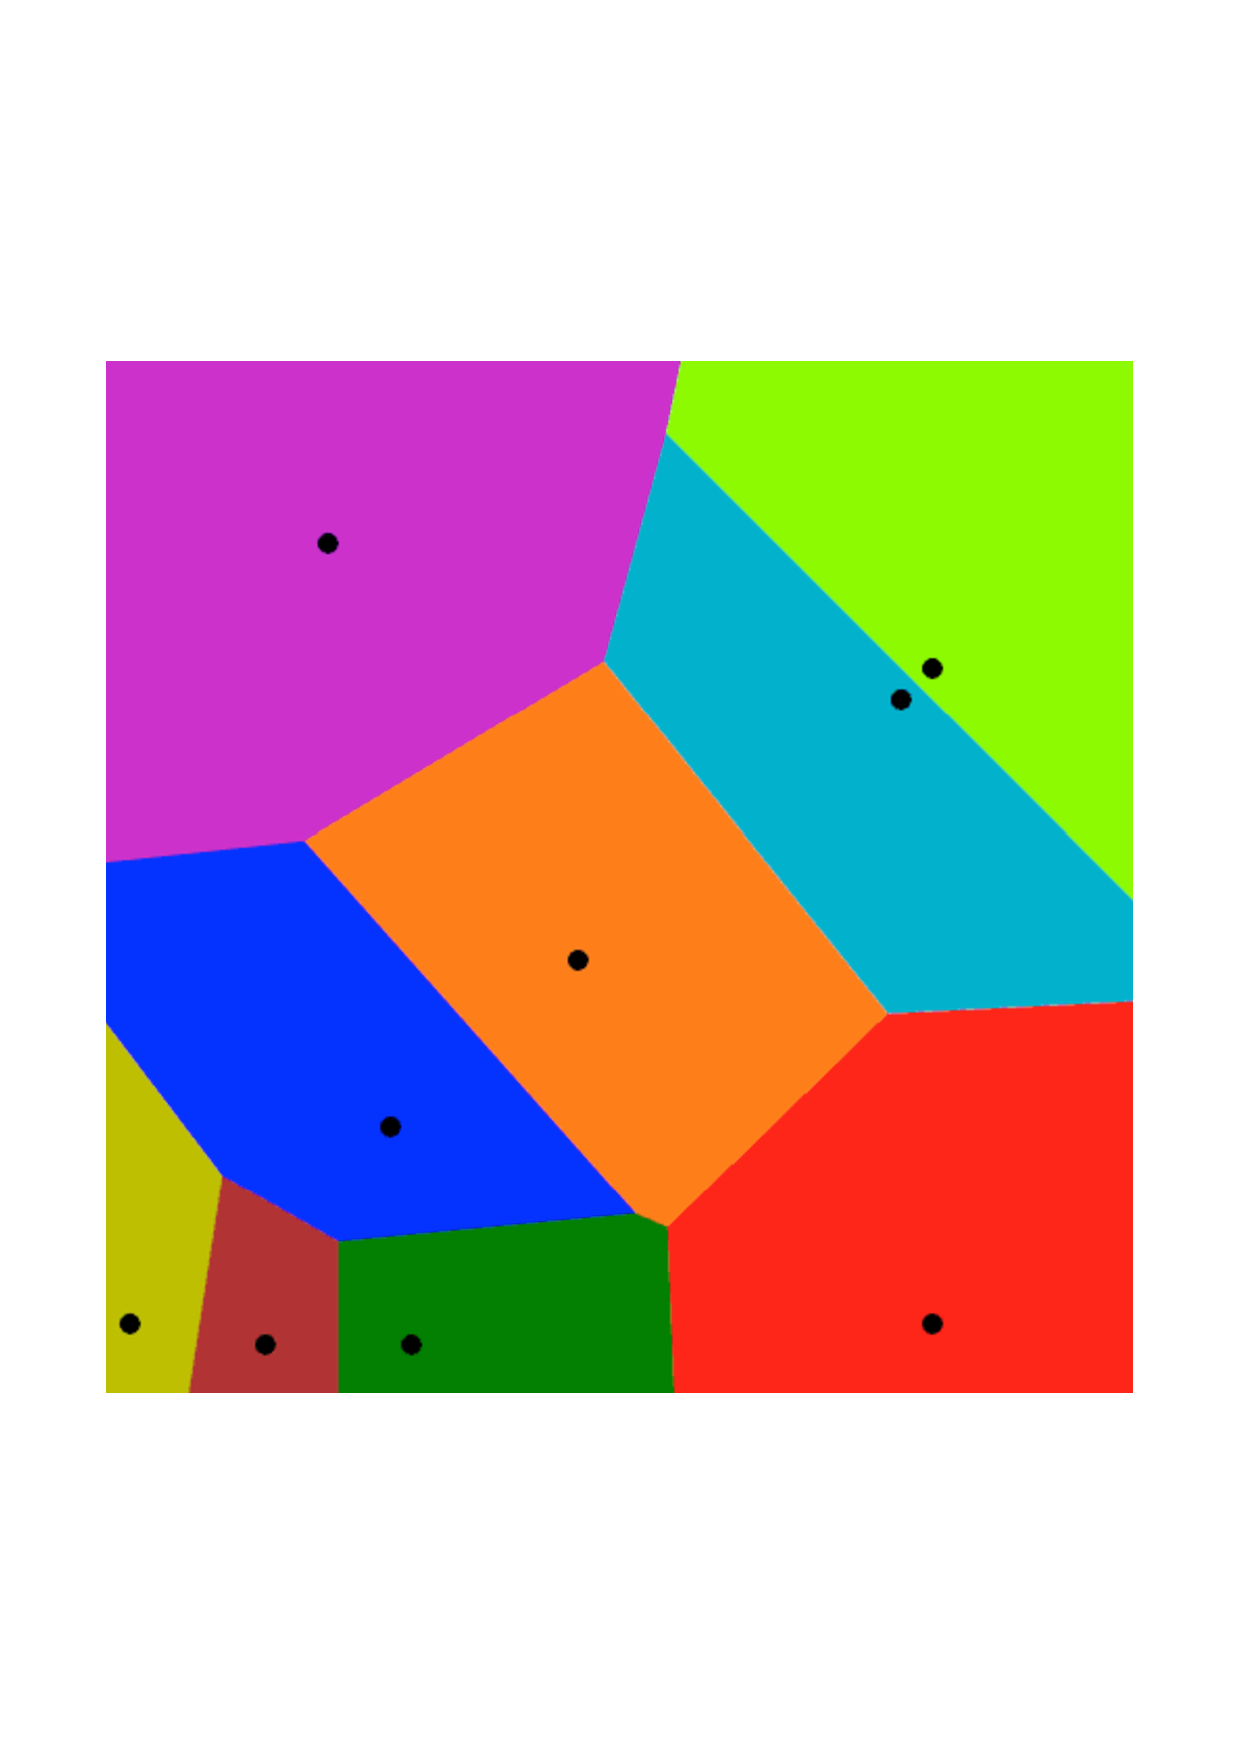
\includegraphics[width=0.4\textwidth]{figures/Voronoi.pdf}
	\end{figure}
	\begin{itemize}
		\item Traditional Voronoi tessellation can be problematic for molecules \pause
		\item Electron density is equally distributed in covalent bonds
		      \begin{itemize}\normalsize
			      \item No electronegativity and bond polarization
		      \end{itemize}
	\end{itemize}
\end{frame}
%%%%%%%%%%%%%%%%%%%%%%%%%%%%%%%%%%%%%%%%%%%%%%%%%%%%%%%%%%%%%%%%%
\begin{frame}
	\frametitle{Radical Voronoi tessellation}
	\begin{figure}
		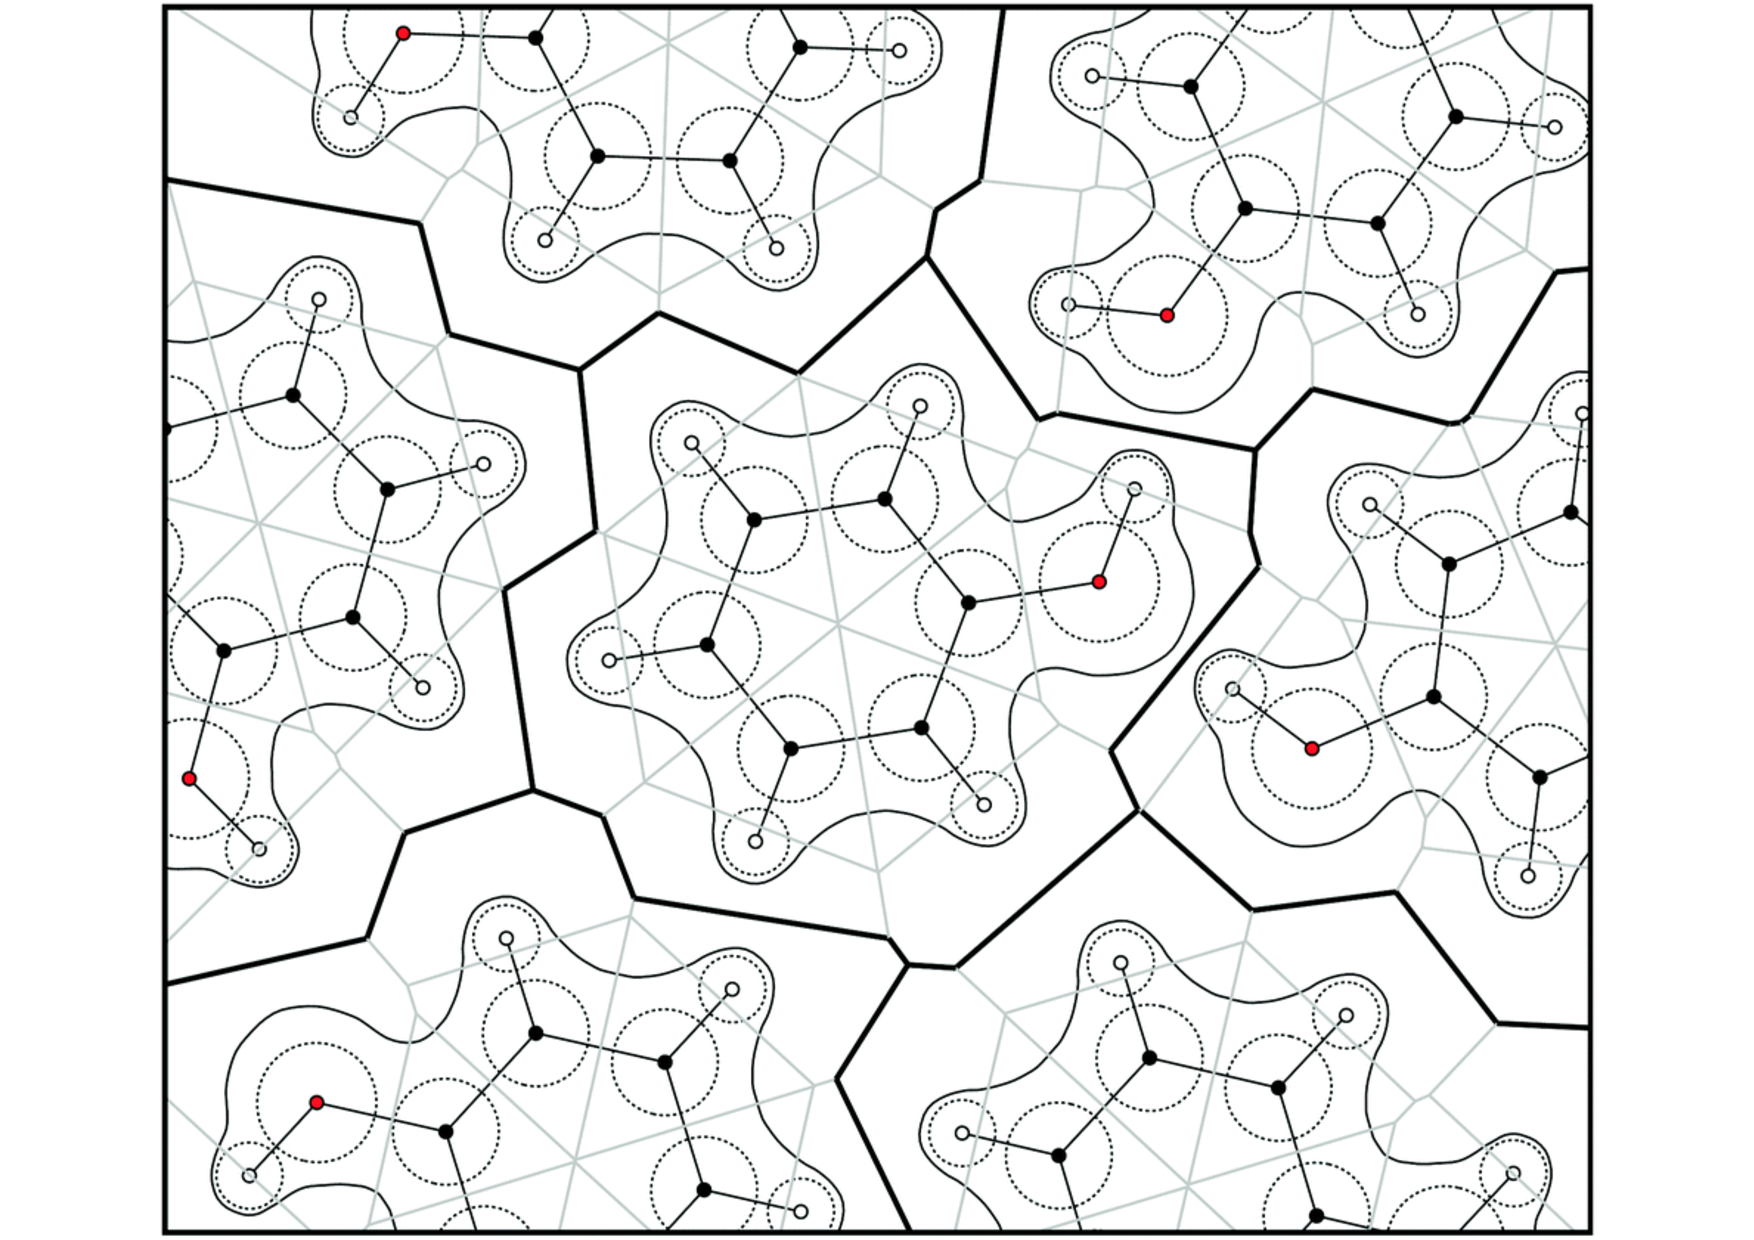
\includegraphics[width=0.55\textwidth]{figures/MT_voronoi.pdf}
	\end{figure}
	\begin{itemize}
		\item radical Voronoi tessellation assigns radii $r_i$ to each site
		      \begin{align*}
			      C_i^r = \{ \mathbf{x} \in \mathbb{R}^3 \, | ( \mathbf{x} - \mathbf{s}_i )^2 - r_i^2 \leq ( \mathbf{x} - \mathbf{s}_j )^2 - r_j^2 \, \forall \, j \neq i \}; i,j=1,...,n
		      \end{align*}
	\end{itemize}
\end{frame}
%%%%%%%%%%%%%%%%%%%%%%%%%%%%%%%%%%%%%%%%%%%%%%%%%%%%%%%%%%%%%%%%%
\begin{frame}
	\frametitle{Radical Voronoi tessellation}
	\begin{figure}
		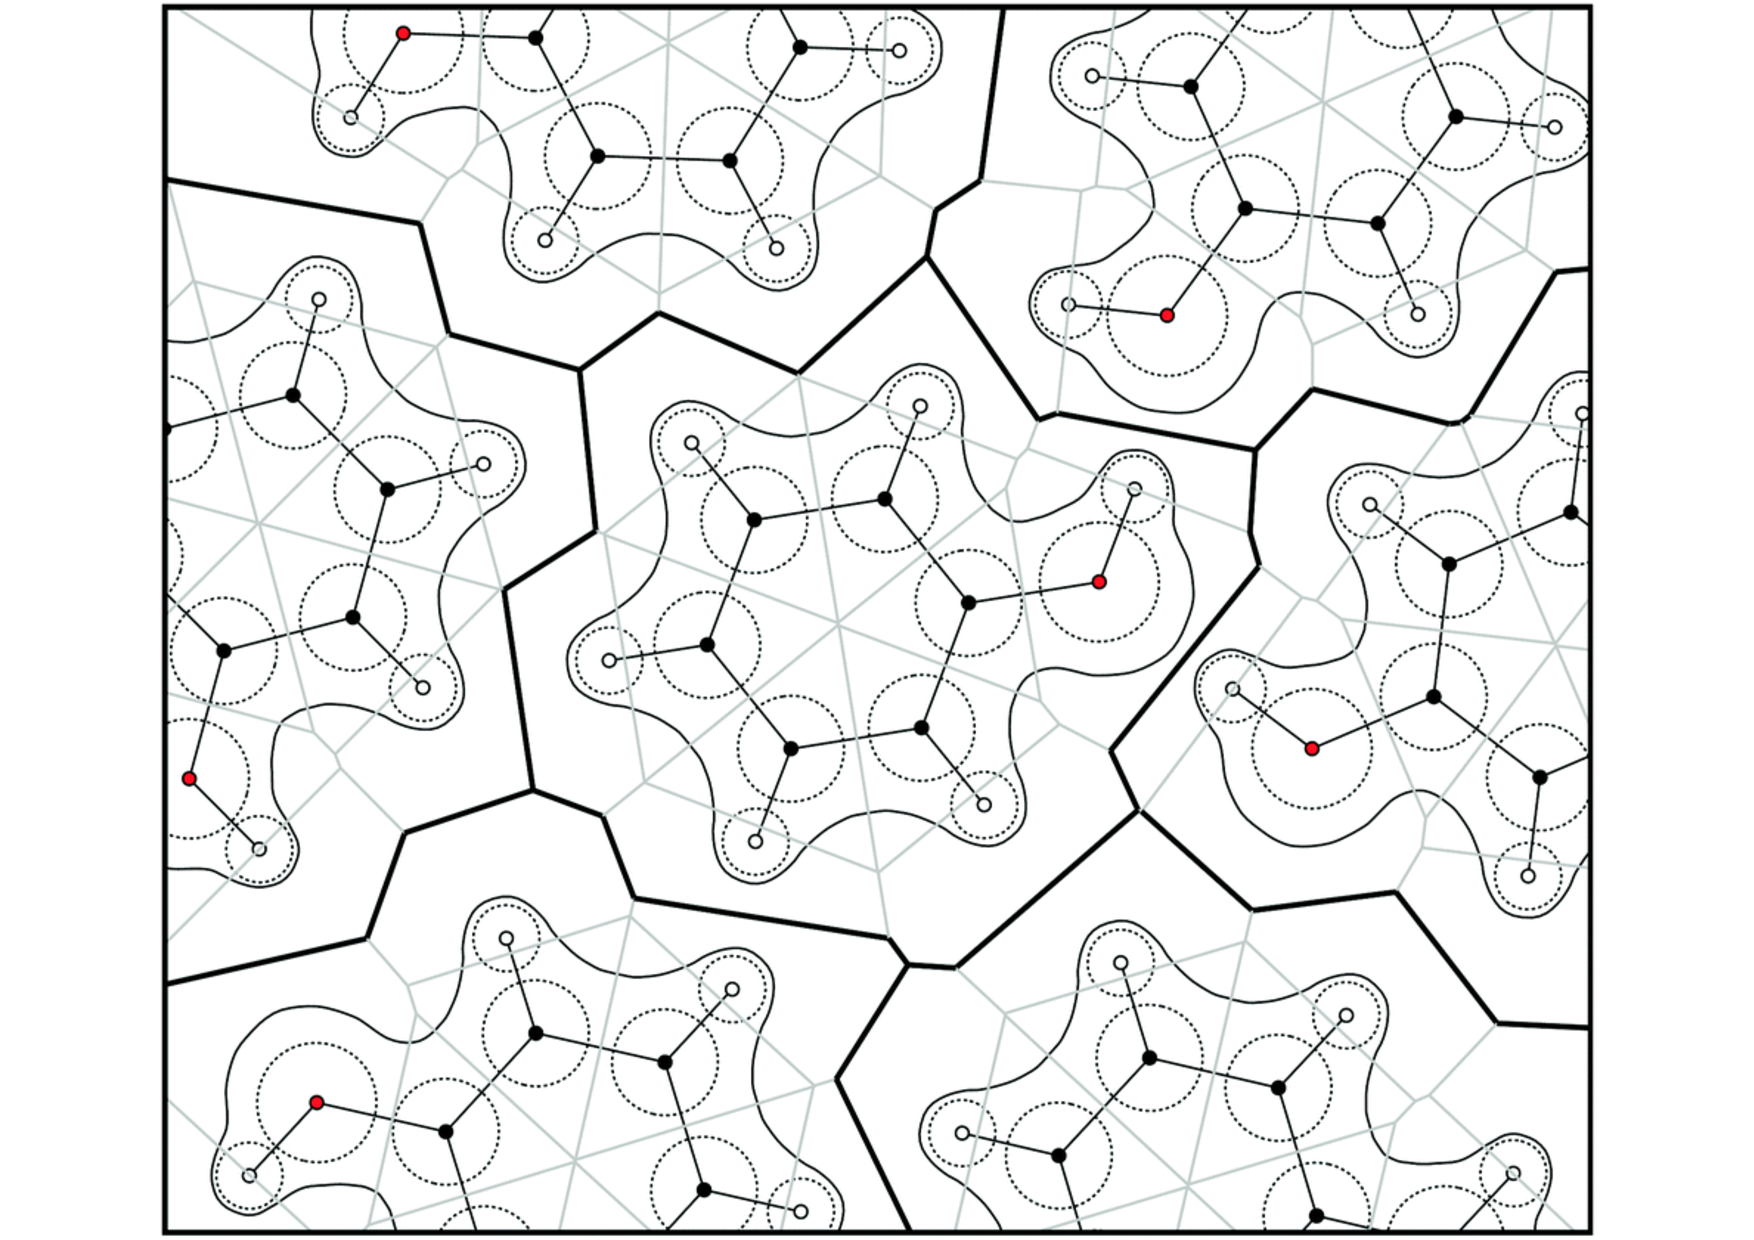
\includegraphics[width=0.55\textwidth]{figures/MT_voronoi.pdf}
	\end{figure}
	\begin{itemize}
		\item merge atomic cells to molecular cells
		\item integrate electron density in molecular cells to obtain molecular dipole moments
	\end{itemize}
	\begin{align*}
		\boldsymbol\upmu_k = \int_{M_k} \mathbf{r} \rho(\mathbf{r}) \mathsf{d}\mathbf{r}
	\end{align*}
\end{frame}
%%%%%%%%%%%%%%%%%%%%%%%%%%%%%%%%%%%%%%%%%%%%%%%%%%%%%%%%%%%%%%%%%
\begin{frame}
	\frametitle{IR and Raman spectra of benzene}
	\vspace{-.6cm}
	\begin{columns}
		\column{0.45\textwidth}
		\begin{figure}
			\vspace{-.6cm}
			\includegraphics[width=1.1\textwidth]{figures/benzene_spectra.png}
		\end{figure}
		\column{0.55\textwidth}
		\vspace{2.5cm}
		\begin{itemize}
			\item Compare Voronoi and Wannier, what do you recognize?
		\end{itemize}
	\end{columns}
\end{frame}
%%%%%%%%%%%%%%%%%%%%%%%%%%%%%%%%%%%%%%%%%%%%%%%%%%%%%%%%%%%%%%%%%
\begin{frame}
	\frametitle{IR and Raman spectra of benzene}
	\vspace{-.6cm}
	\begin{columns}
		\column{0.45\textwidth}
		\begin{figure}
			\vspace{-.6cm}
			\includegraphics[width=1.1\textwidth]{figures/benzene_spectra2.png}
		\end{figure}
		\column{0.55\textwidth}
		\begin{itemize}
			\item \textbf{IR}: Wannier predicts additional bands between 1200~cm$^{-1}$ and 1350~cm$^{-1}$
			\item[]
			      $\rightarrow$ symmetry breaking by Wannier functions, localization produces alternating single and double bonds in the ring
			\item[]
			      $\rightarrow$ Wannier function centers are regularly interchanging in the trajectory causing artificial dipole moment changes
		\end{itemize}
		\begin{figure}
			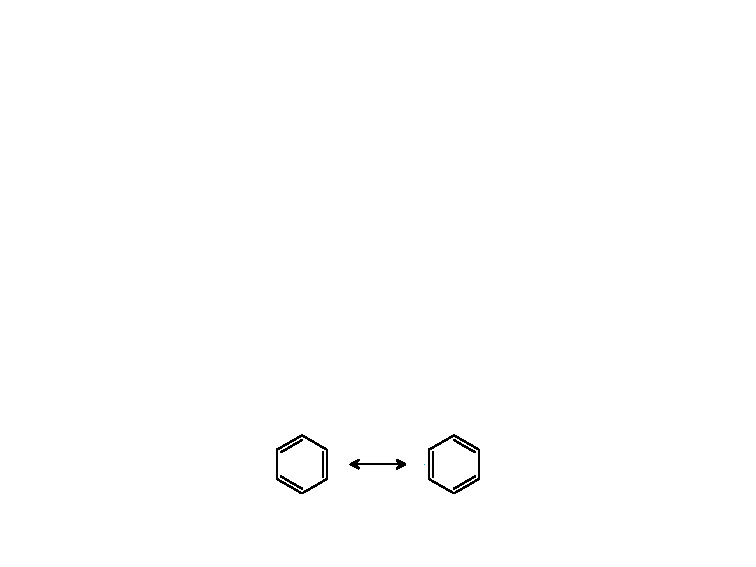
\includegraphics[width=.6\textwidth]{figures/benzene_mesomerie.pdf}
		\end{figure}
	\end{columns}
\end{frame}
%%%%%%%%%%%%%%%%%%%%%%%%%%%%%%%%%%%%%%%%%%%%%%%%%%%%%%%%%%%%%%%%%
\begin{frame}
	\frametitle{IR and Raman spectra of benzene}
	\vspace{-.6cm}
	\begin{columns}
		\column{0.45\textwidth}
		\begin{figure}
			\vspace{-.6cm}
			\includegraphics[width=1.1\textwidth]{figures/benzene_spectra2.png}
		\end{figure}
		\column{0.55\textwidth}
		\begin{itemize}
			\item \textbf{Raman}: Wannier does not produce a useful spectrum
			\item[]
			      $\rightarrow$ polarizabilities are obtained by electronic structure calculations with and without an external electric field
			\item[]
			      $\rightarrow$ localization algorithm does not converge to same bond pattern in the two electronic structure calculations
			\item[]
			      $\rightarrow$ polarizability artificially increased by orders of magnitude
		\end{itemize}
	\end{columns}
\end{frame}
%%%%%%%%%%%%%%%%%%%%%%%%%%%%%%%%%%%%%%%%%%%%%%%%%%%%%%%%%%%%%%%%%
\begin{frame}
	\frametitle{Vibrational circular dichroism}
	\begin{itemize}
		\item measures differential absorbance of left- and right-circularly polarized infrared radiation during vibrational transitions
		      \begin{align*}
			      \Delta A = A_\mathsf{L} - A_\mathsf{R}
		      \end{align*}
		\item for chiral molecules $\Delta A$ is unequal to zero
		\item enantiomers show either a positive or negative band for each vibrational mode
	\end{itemize}
\end{frame}
%%%%%%%%%%%%%%%%%%%%%%%%%%%%%%%%%%%%%%%%%%%%%%%%%%%%%%%%%%%%%%%%%
\begin{frame}
	\frametitle{Vibrational circular dichroism}
	\begin{figure}
		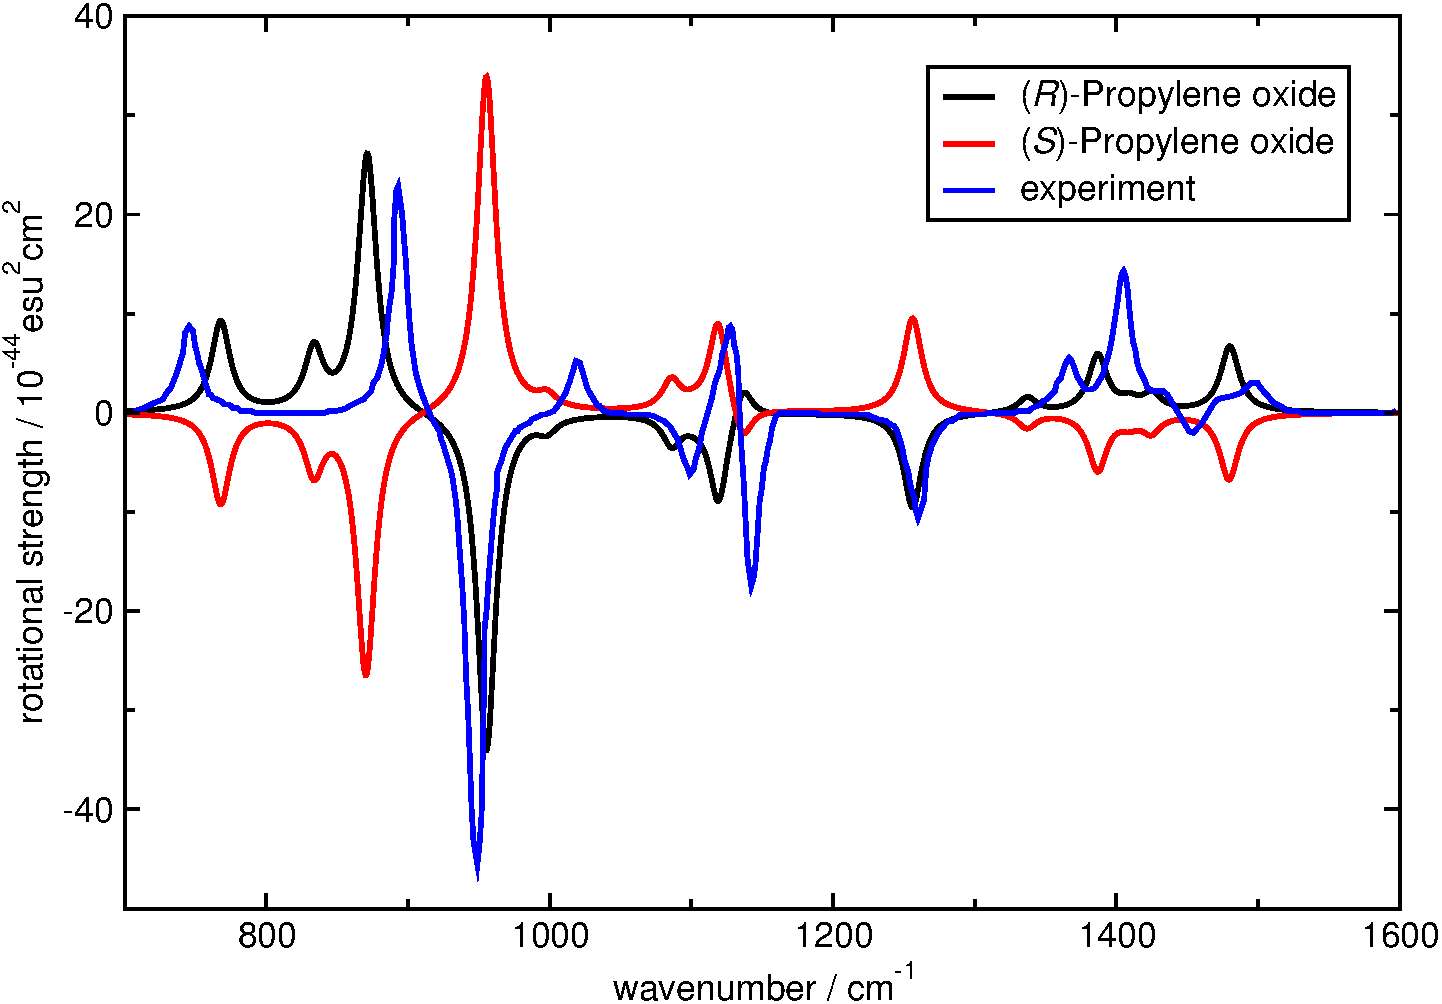
\includegraphics[width=.8\textwidth]{figures/PropOx_vcd.pdf}
	\end{figure}
\end{frame}
%%%%%%%%%%%%%%%%%%%%%%%%%%%%%%%%%%%%%%%%%%%%%%%%%%%%%%%%%%%%%%%%%
\begin{frame}
	\frametitle{Vibrational circular dichroism}
	\begin{itemize}
		\item measures differential absorbance of left- and right-circularly polarized infrared radiation during vibrational transitions
		      \begin{align*}
			      \Delta A = A_\mathsf{L} - A_\mathsf{R}
		      \end{align*}
		\item for chiral molecules $\Delta A$ is unequal to zero
		\item enantiomers show either a positive or negative band for each vibrational mode
		\item \textbf{Correlation function:}
		      \begin{align*}
			      \Delta A (\tilde{\nu}) \propto \int \biggl[\langle \dot{\bmu} (\tau) \cdot \dot{\boldsymbol{\mathsf{m}}} (t + \tau) \rangle_{\tau} - \langle \dot{\boldsymbol{\mathsf{m}}} (\tau) \cdot \dot{\bmu} (t + \tau) \rangle_{\tau} \biggl] \mathsf{e}^{-2\pi i c \tilde{\nu} t}\mathsf{d}t
		      \end{align*}
	\end{itemize}
\end{frame}
%%%%%%%%%%%%%%%%%%%%%%%%%%%%%%%%%%%%%%%%%%%%%%%%%%%%%%%%%%%%%%%%%
\begin{frame}
	\frametitle{Thomas--Kirchner approach}
	\begin{itemize}
		\item classical expression for magnetic dipole moment $\mathbf{m}$
		      \begin{align*}
			      \mathbf{m} = \frac{1}{2} \int \mathbf{r} \times \mathbf{j}(\mathbf{r}) \mathsf{d}\mathbf{r}
		      \end{align*}
		      \pause
		\item changes in electron density act as source for electric current
		      \begin{align*}
			      \frac{\partial \rho (\mathbf{r},t)}{\partial t} + \nabla \mathbf{j}(\mathbf{r},t) = 0
		      \end{align*}
		      \pause
		\item electric current density is product of electron density and scalar field
		      \begin{align*}
			      \mathbf{j}(\mathbf{r},t) = -\rho (\mathbf{r},t) \nabla \alpha(\mathbf{r},t)
		      \end{align*}
	\end{itemize}
\end{frame}
%%%%%%%%%%%%%%%%%%%%%%%%%%%%%%%%%%%%%%%%%%%%%%%%%%%%%%%%%%%%%%%%%
\begin{frame}
	\frametitle{Thomas--Kirchner approach}
	\begin{itemize}
		\item combining both conditions yields differential equation
		      \begin{align*}
			      \frac{\partial \rho (\mathbf{r},t)}{\partial t} = \nabla \rho (\mathbf{r},t) \cdot \nabla \alpha (\mathbf{r},t) + \rho(\mathbf{r},t) \Delta \alpha(\mathbf{r},t)
		      \end{align*}
		\item solve to obtain scalar field $\alpha(\mathbf{r},t)$
	\end{itemize}
	\begin{figure}
		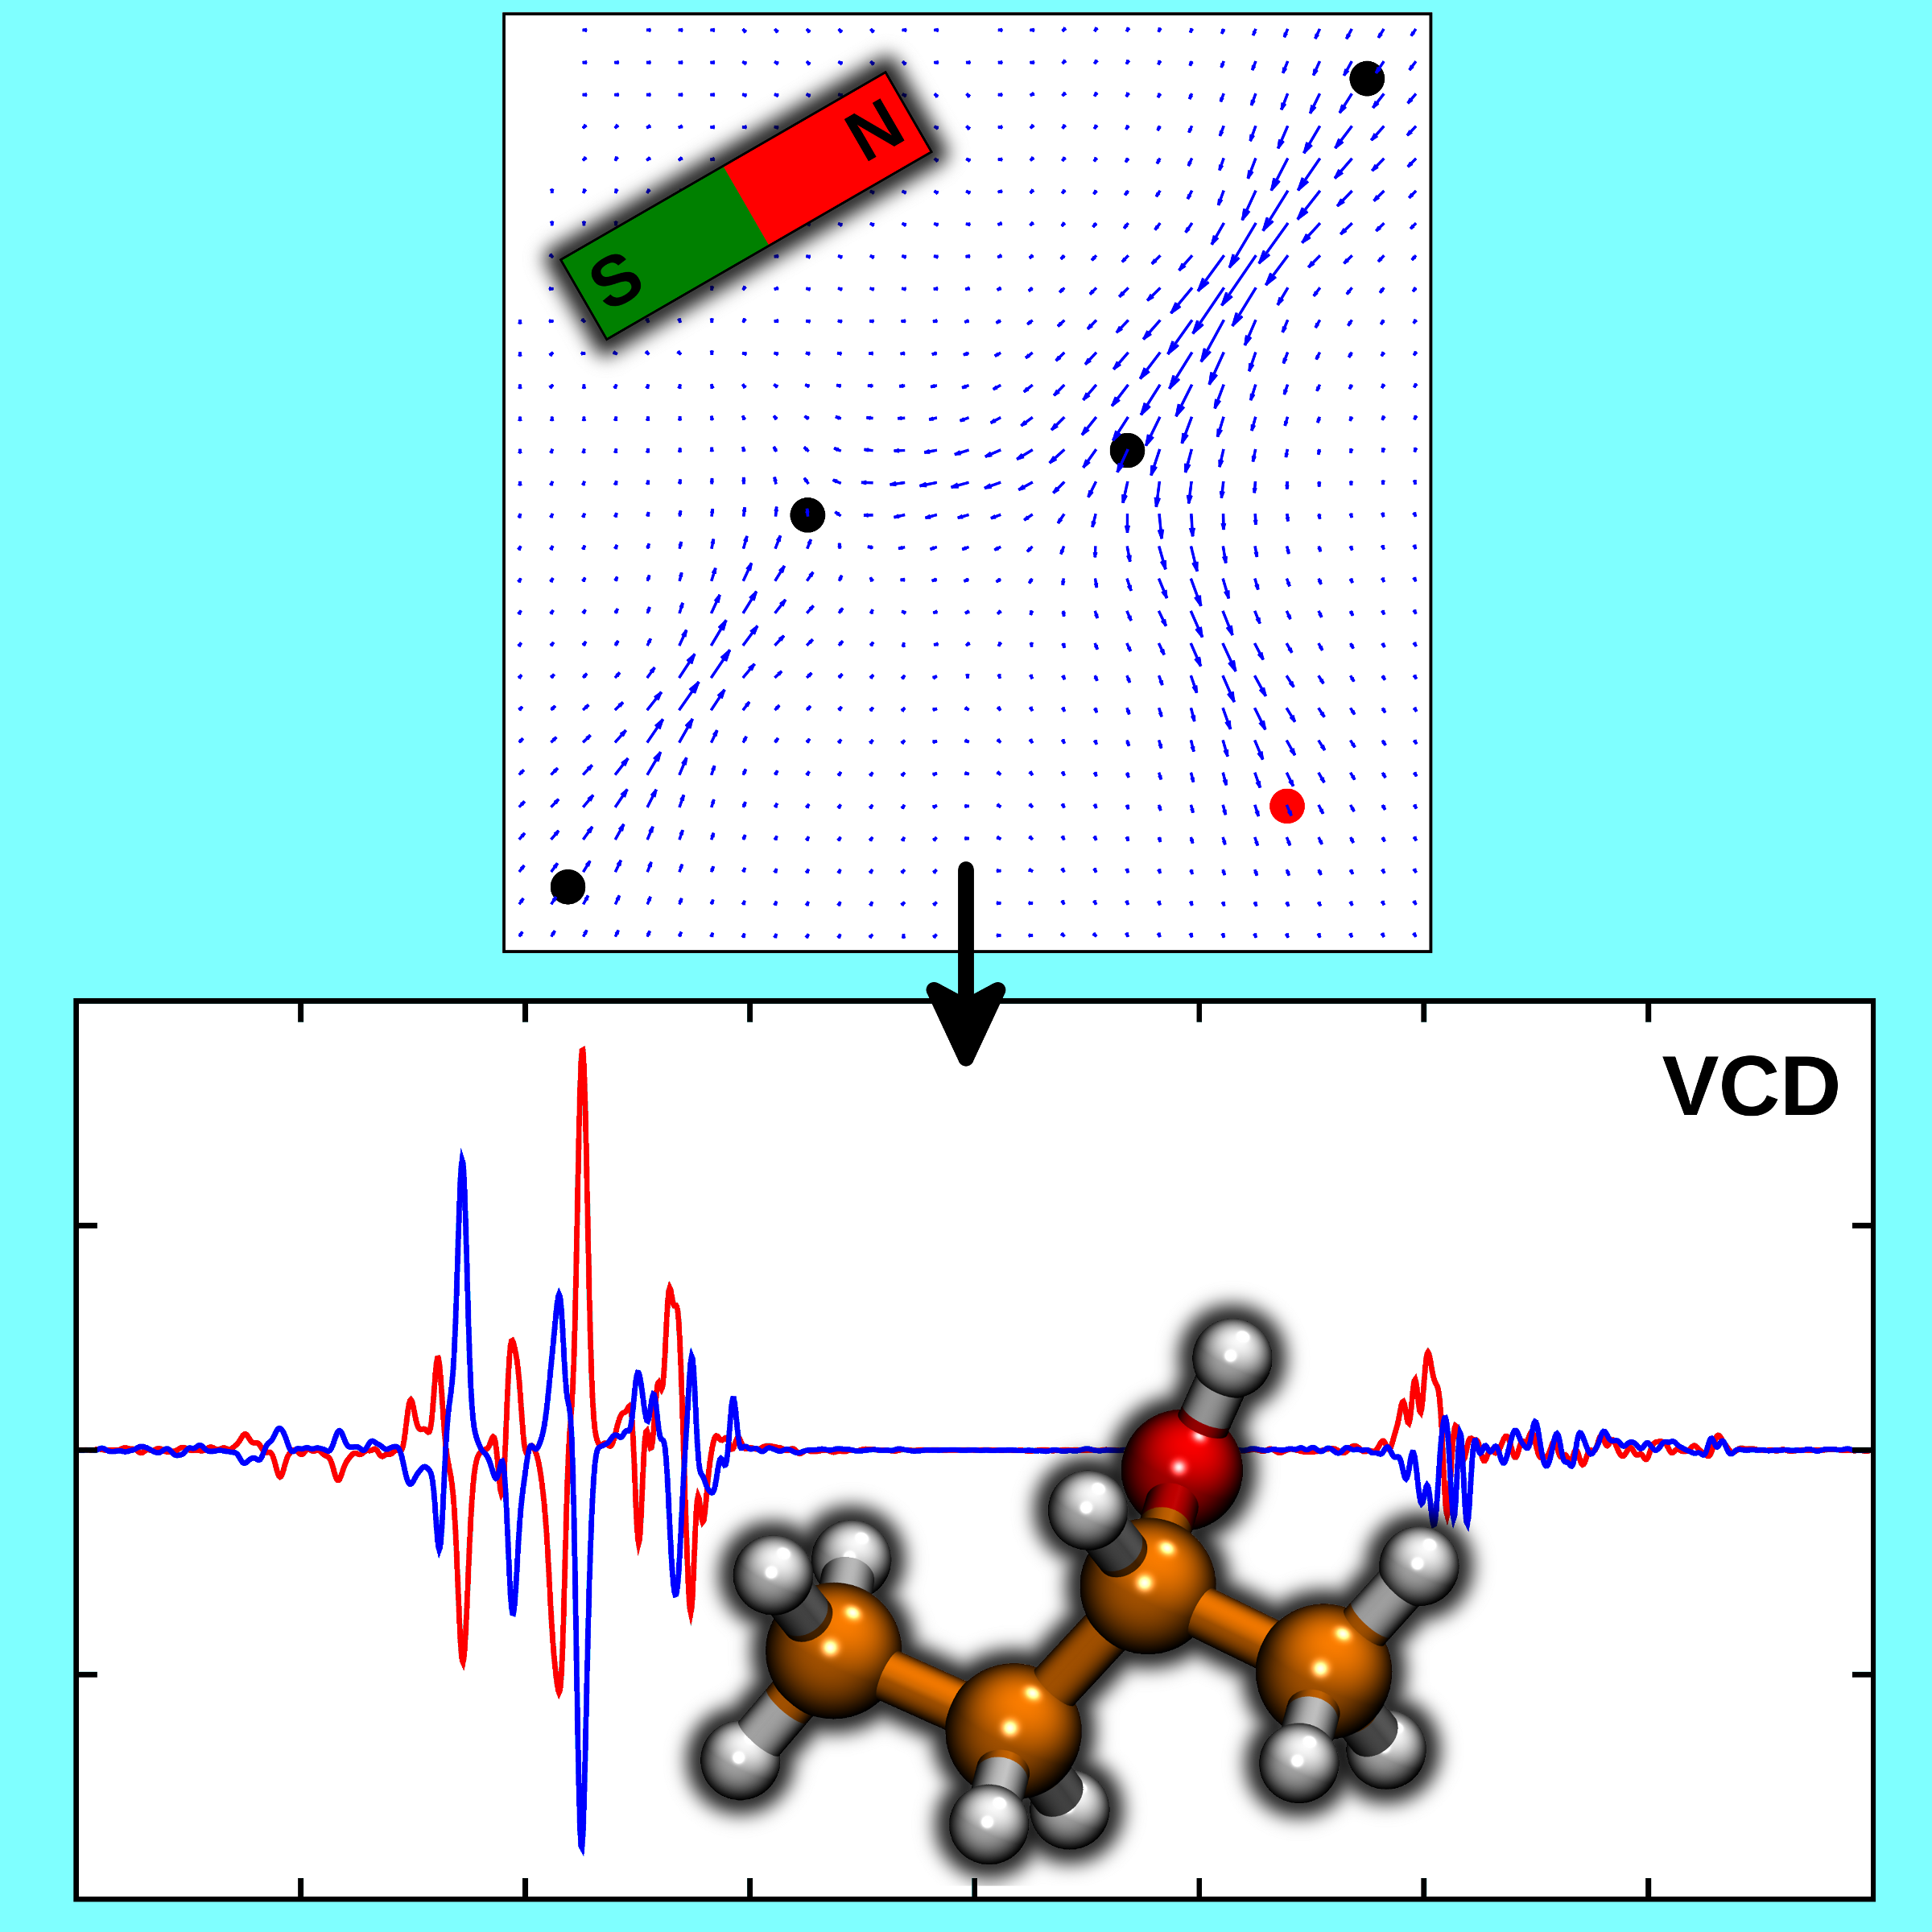
\includegraphics[width=.38\textwidth]{figures/MT_TOC.png}
	\end{figure}
\end{frame}
%%%%%%%%%%%%%%%%%%%%%%%%%%%%%%%%%%%%%%%%%%%%%%%%%%%%%%%%%%%%%%%%%
\begin{frame}
	\frametitle{Thomas--Kirchner approach}
	\vspace{-.25cm}
	\begin{columns}
		\column{.5\textwidth}\centering
		\textbf{Gas phase}
		\vspace{-.25cm}
		\begin{figure}
			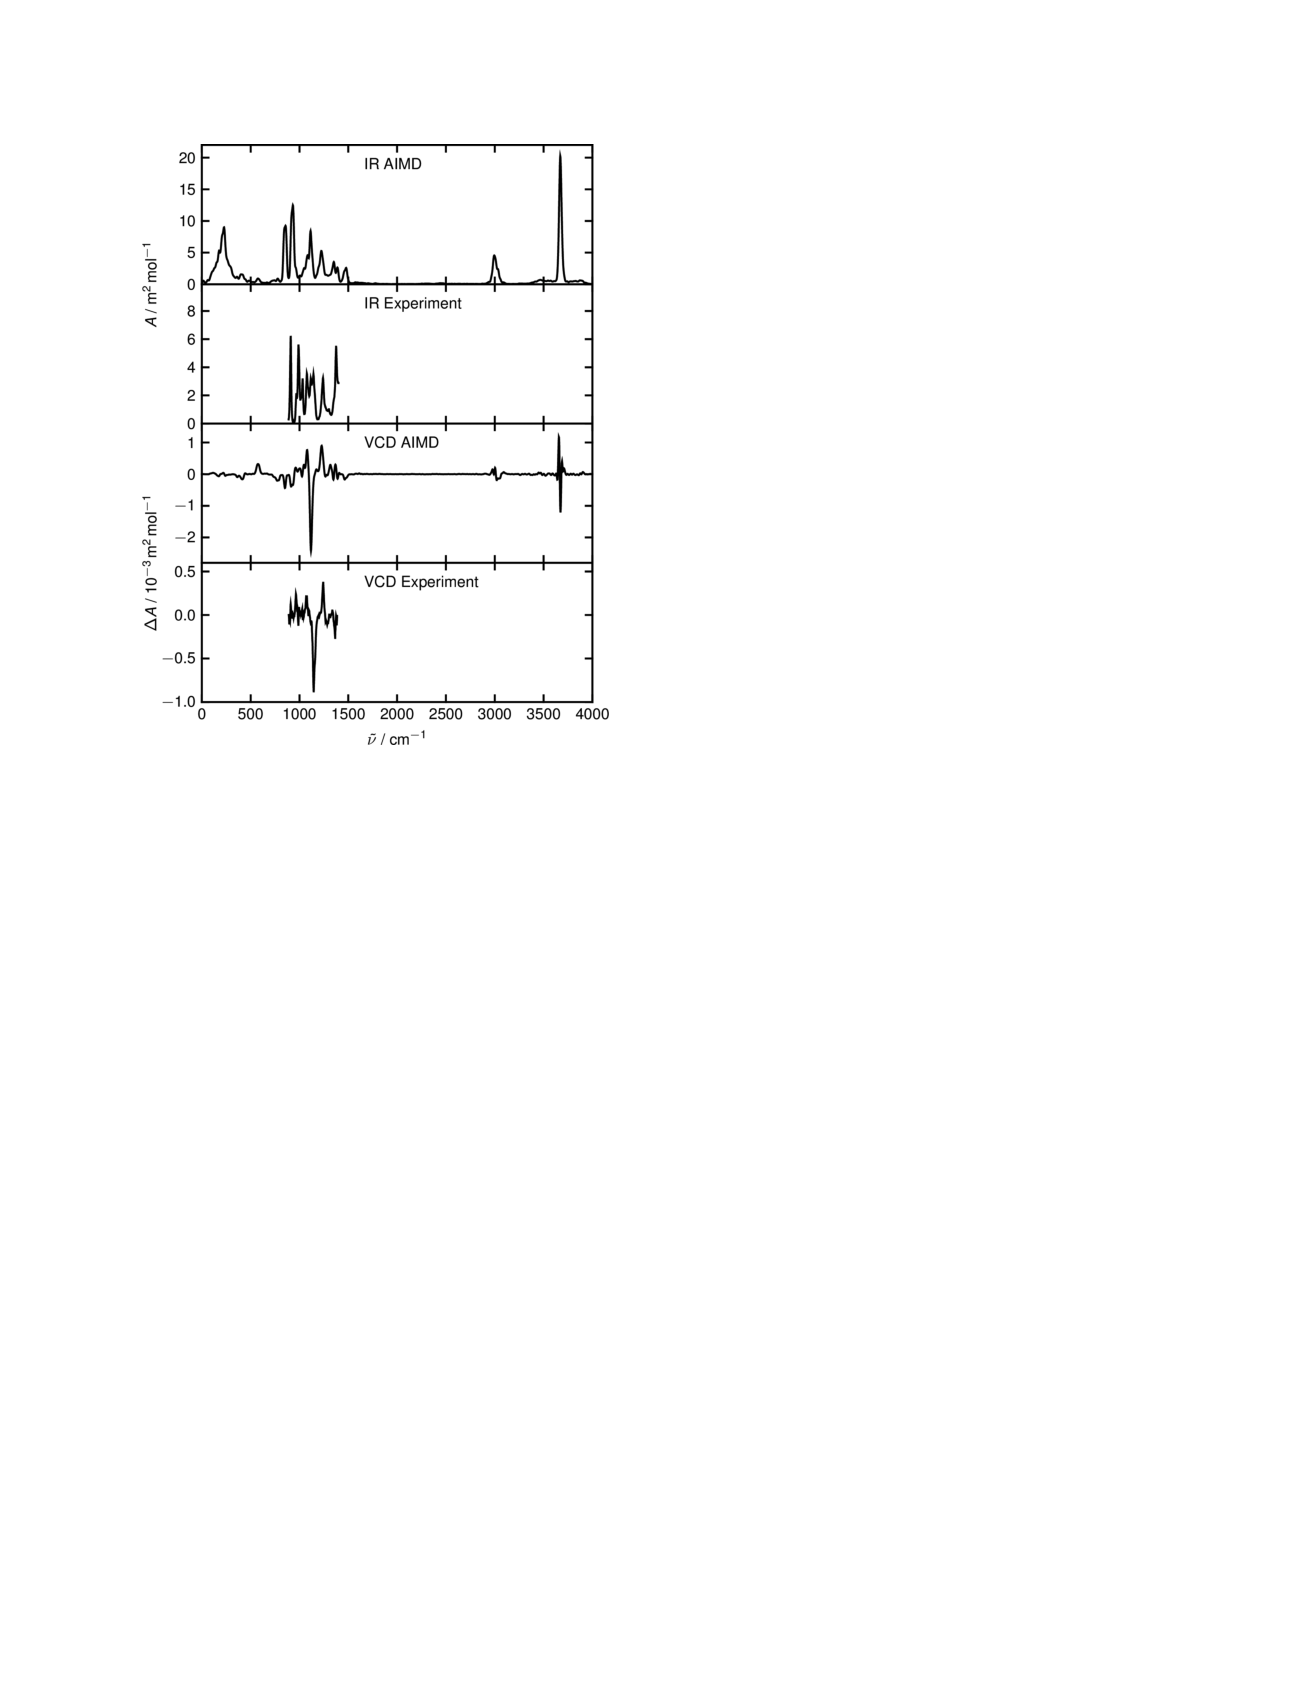
\includegraphics[width=.95\textwidth]{figures/butanol_gas_vcd.pdf}
		\end{figure}
		\column{.5\textwidth}\centering
		\textbf{Bulk phase}
		\vspace{-.25cm}
		\begin{figure}
			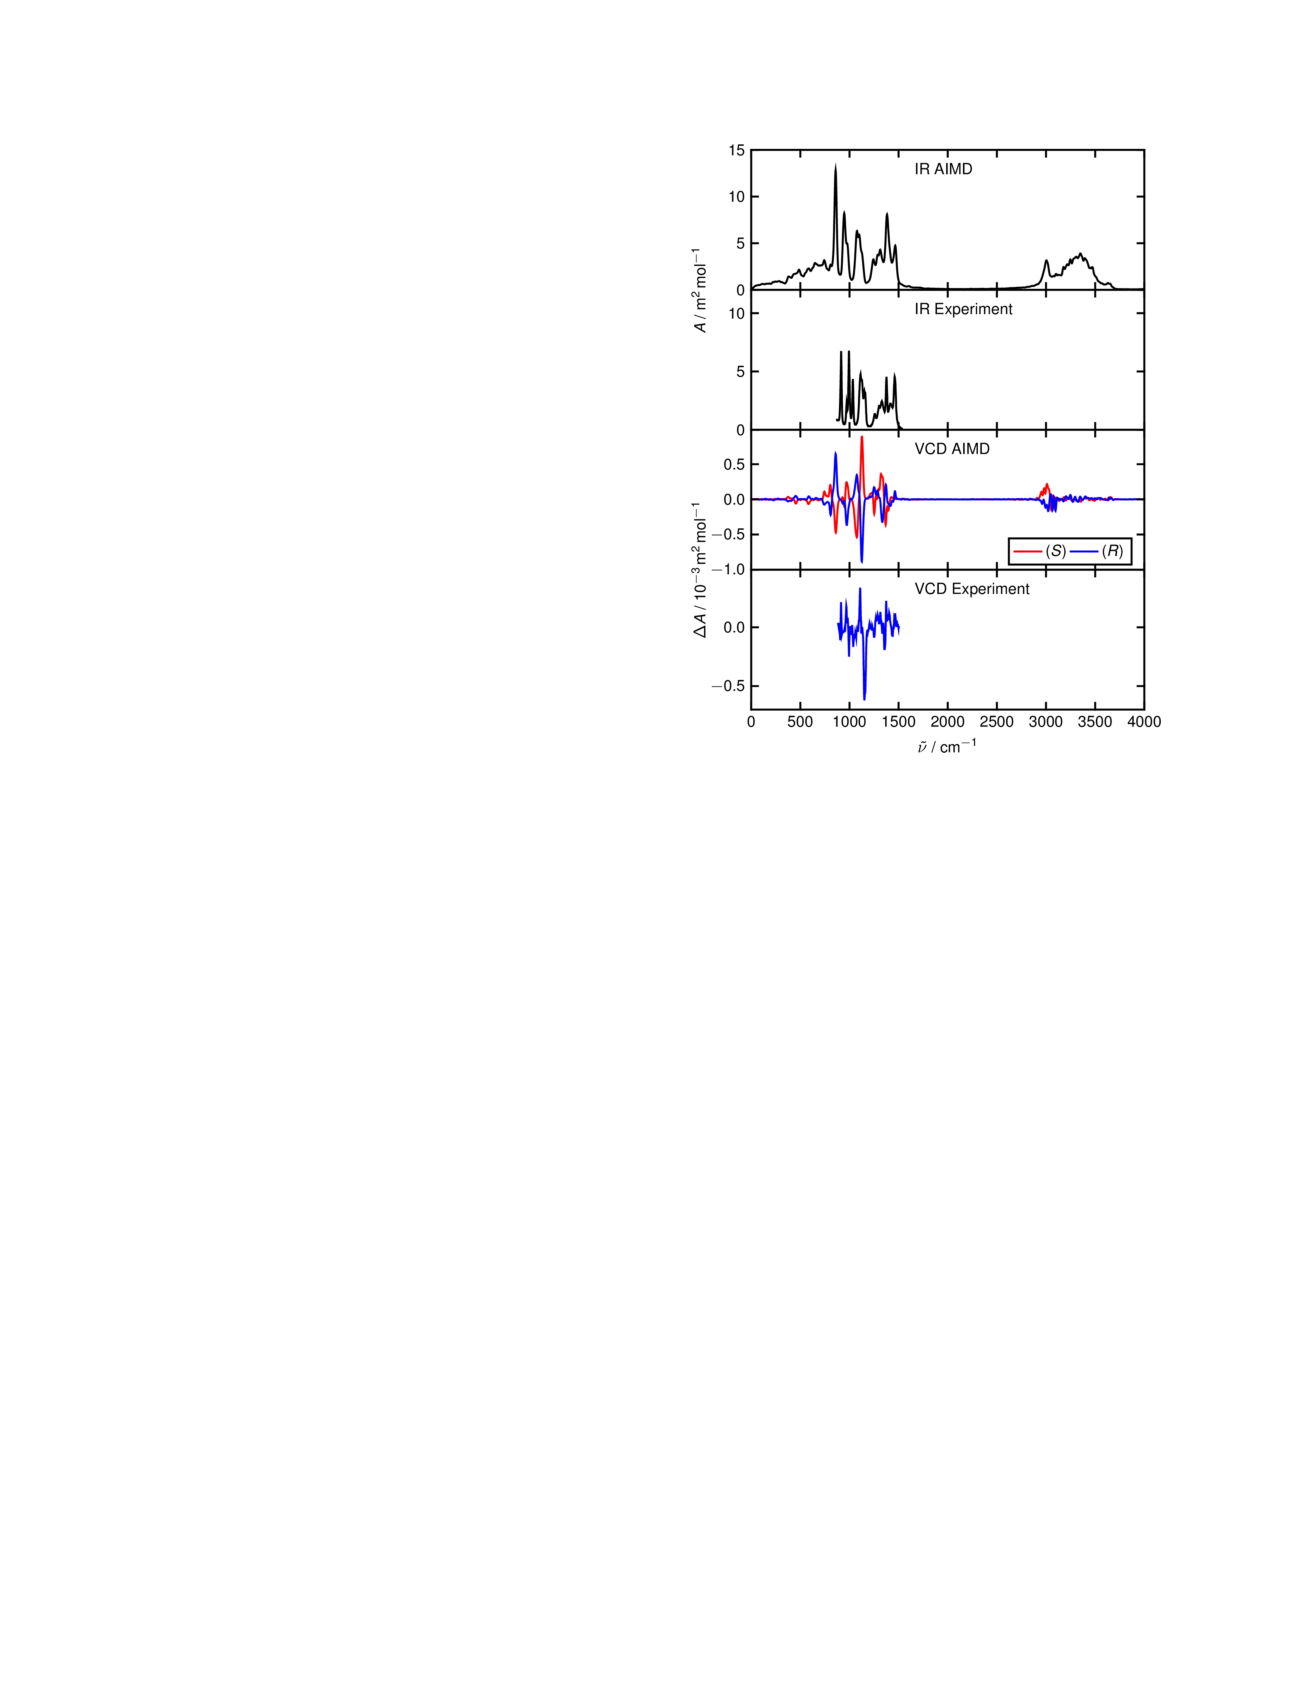
\includegraphics[width=.95\textwidth]{figures/butanol_bulk_vcd.pdf}
		\end{figure}
	\end{columns}
\end{frame}
%%%%%%%%%%%%%%%%%%%%%%%%%%%%%%%%%%%%%%%%%%%%%%%%%%%%%%%%%%%%%%%%%
\begin{frame}{Summary: Vibrational spectroscopy}
	\begin{enumerate}
		\item Static approach (QM)
		      \begin{itemize}
			      \item Solve stationary Schrödinger equation
			      \item Represent all vibrational modes as harmonic oscillators
			      \item[$+$] High accuracy and fast (DFT)
			      \item[$+$] Implemented in many QM codes
			      \item[$-$] Small region around (global) minimum geometry is modelled
			      \item[$-$] Only electronic ground state
		      \end{itemize}
		\item Dynamic approach (MD)
		      \begin{itemize}
			      \item Express vibrational spectra by correlation functions
			      \item[$+$] Better sampling of the PES
			      \item[$+$] Good for liquid systems and solvation
			      \item[$-$] Computationally demanding
			      \item[$-$] Reliable dipole moments and polarizabilities required (e.g. Wannier does not work for aromatic systems)
		      \end{itemize}
	\end{enumerate}
\end{frame}
%%%%%%%%%%%%%%%%%%%%%%%%%%%%%%%%%%%%%%%%%%%%%%%%%%%%%%%%%%%%%%%%%
\end{document}